%%%%%%%%%%%%%%%%%%%%%%%%%%%%%%%%%%%%%%%%%%%%%%%%%%%%%%%%%%%%%%%%%%% 
%                                                                 %
%                            CHAPTER SIX                          %
%                                                                 %
%%%%%%%%%%%%%%%%%%%%%%%%%%%%%%%%%%%%%%%%%%%%%%%%%%%%%%%%%%%%%%%%%%% 
\chapter{SEMANTIC IMPORTANCE GENERALIZATION AND BENCHMARK}
The sequential stream reasoning architecture (SSRA) is an innovative architecture that is designed and implemented specifically for stream reasoning use cases aiming to mine the knowledge in the boundless and torrent streaming data. 
Based on SSRA, two use cases are implemented, which to some extent demonstrates the usefulness of the semantic importance in the stream reasoning context. 
However, SSRA implementations are evaluated out of commercial triple-store products, where only three strategies and a few of semantic importance aspects are included.
In the use case implementations, specific case-by-case assumptions are applied. 
Even though the experimental results have shown some evidence to support the advancement of the semantic importance, they are still not sufficient to describe how semantic importance can bring values to the stream reasoning, as well as be generally applied to a wide range of stream reasoning applications.

This chapter provides a comprehensive view of the usefulness and reusability for the concept of semantic importance.
The core contribution in this chapter is a generalization and benchmark framework called \textbf{SIGenBench}. 
It generalizes semantic importance by connecting it to the state-of-the-art stream reasoning techniques.
It also features a flexible benchmark system that can be configured to adapt with different stream reasoning scenarios. 
This benchmark reports four system key performance metrics including memory consumption, response time, precision, and throughput, with which the impacts and benefits of semantic importance are discussed in details.  
%
\section{Introduction}
Figure \ref{fig:6-sib} shows the architecture of SIGenBench.
SIGenBench is implemented based on SSRA, and provides two main functionalities: generalization (blue) and benchmark (green).
Generalization refers to reusability, i.e. how semantic importance can be reused in different use cases.
Benchmark refers to usefulness, i.e. how semantic importance can be useful in various stream reasoning settings.

\begin{figure}[!htbp]
	\centering
    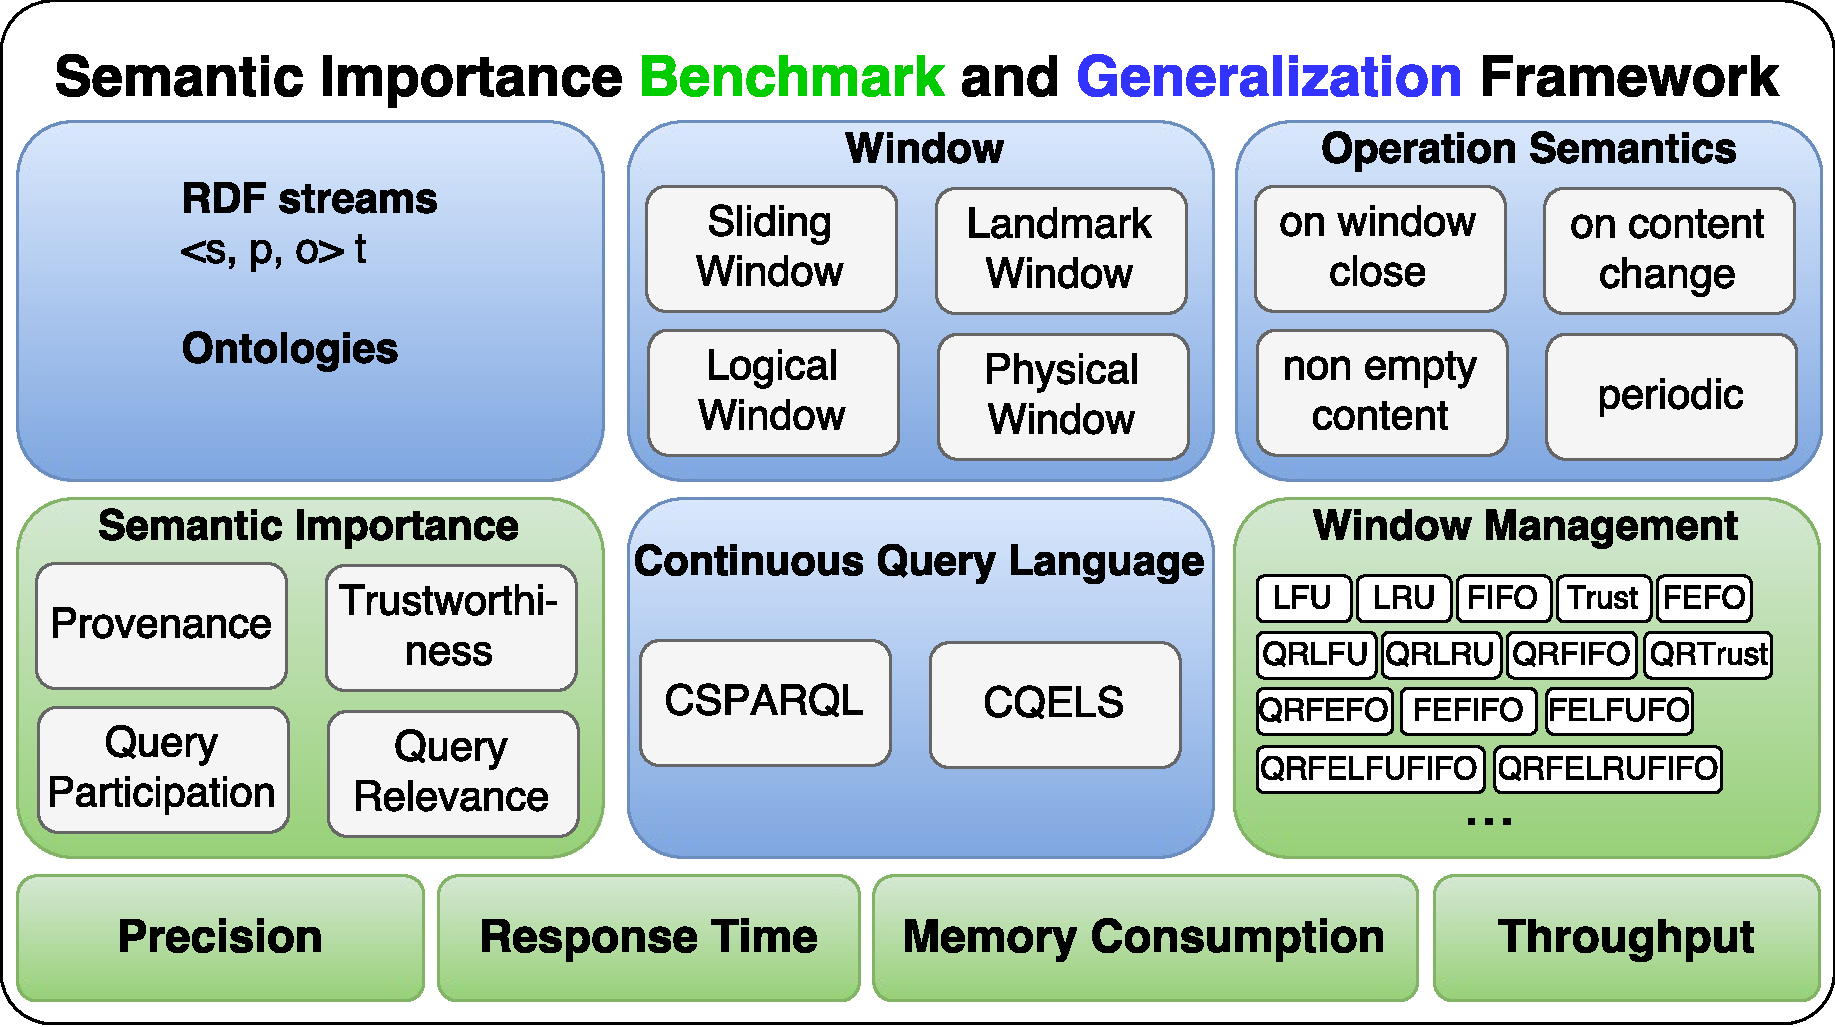
\includegraphics[width=5in]{img/6-sib.pdf}
    \caption{SIGenBench Architecture}
    \label{fig:6-sib}
\end{figure}

In order to enable generalization, semantic importance ontology (SIO) is created.
SIO is a descriptive ontology that extends the Prov-O ontology \cite{lebo2013prov}. 
It encodes all the current aspects, and is grounded with real-world example instances, which makes the idea of semantic importance more easier to understand, reuse, and extend. 
SIGenBench also supports popular stream reasoning techniques, such as RDF stream \cite{della2009s}, windows \cite{patroumpas2006window}, report operational semantics \cite{botan2010secret}, as well as continuous query languages \cite{le2011native} \cite{barbieri2009c}.
This enables SIGenBench to be adaptive and flexible when working with various stream reasoning systems. 

In order to enable benchmark, SIGenBench records four performance metrics.
Precision describes how precise the system can be under some window management strategy, the higher the better.
Response time indicates how fast the system can respond under certain window management strategy, the faster the better. 
Memory consumption is measured in terms of the number of streaming data items in the window.
It indicates how scale the system is under one window management strategy, the smaller the better.
Throughput indicates how quickly the system can process the streaming data, which is measured by data items per second, the quicker the better. 
SIGenBench also features 26 built-in window management strategies that are derived from the semantic importance model. 
This benchmark system supports both user-specified data or default data. 
The default data includes a RDF stream generator and a background ontology.
It can be configured to simulate different types of streaming data thus can be used to test semantic importance in different settings. 
%
\section{Generalization}
For the concept of semantic importance to be reusable, it must 
(1) provide a set of infrastructure tools so that the concept can be implemented, extended, and invoked in different applications, 
and (2) connect with the state-of-the-art stream reasoning work, such as RDF stream, continuous queries, window semantics and report operational semantics, etc.
%
\subsection{Semantic Importance Ontology}
Ontologies are portable, expandable, general and expressive.
All the current semantic importance concepts have been implemented in an OWL-encoded ontology via extending PROV-O \cite{lebo2013prov}.
Figure \ref{fig:6-sicr} shows the classes and their relationships in the semantic importance ontology. 
All fonts in blue indicates that they are inherited from PROV-O ontology. 
Both \textbf{QueryRelevance} and \textbf{Trustworthiness} are \textbf{prov:Entity}, but \textbf{QueryParticipation} is a \textbf{prov:Activity}.
For more details, please refer to Appendix A.1. 

\begin{figure}[!htbp]
    \centering
    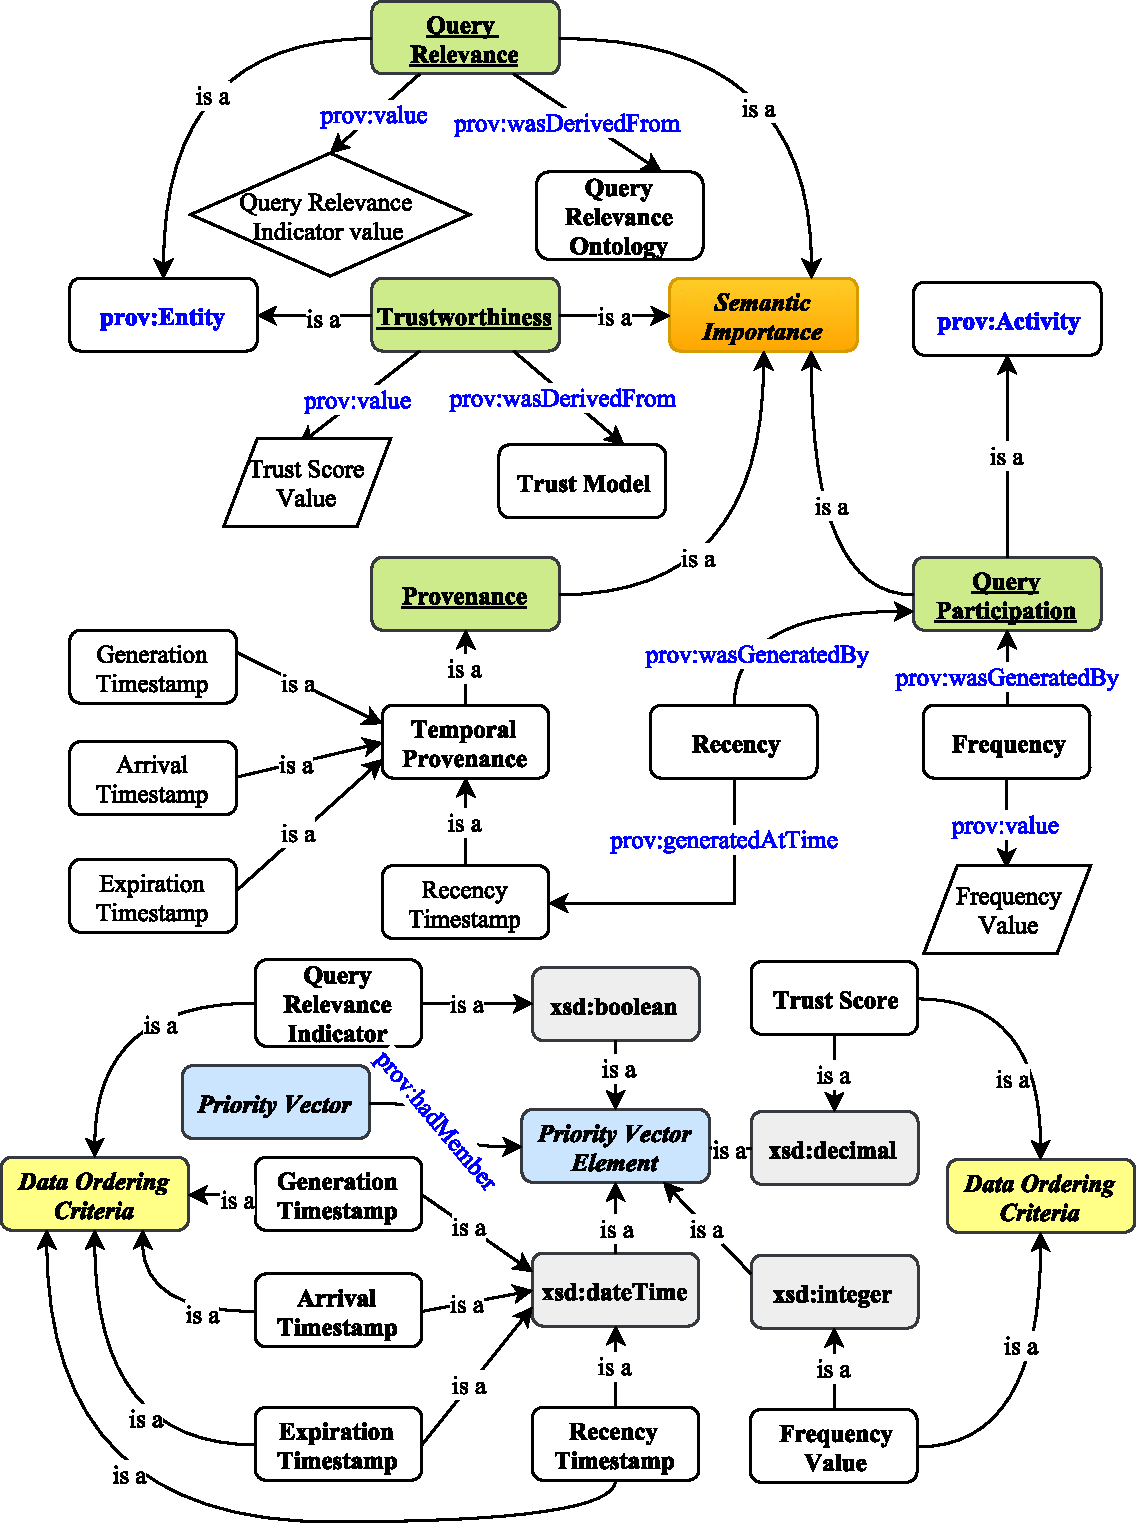
\includegraphics[width=5in]{img/6-sicr.pdf}
    \caption{Semantic Importance Ontology}
    \label{fig:6-sicr}
\end{figure}
%
\subsection{Connection to Stream Reasoning}
SIGenBench is carefully designed in order to embrace both the state-of-the-art and popular stream reasoning techniques.
For instance, SIGenBench is compatible with different continuous query languages and report operational semantics. 
As \cite{dell2013correctness} mentions, the correctness of a stream reasoning engine is critically dependent upon the operational semantics. 
Since different stream reasoning systems can behave differently \cite{botan2010secret}, the benchmark systems aiming to measure the stream reasoning performance should be able to consider the differences in various built-in operational semantics.

SIGenBench decouples the operational semantics from stream reasoning engines.
For example, CSPARQL engine reports when the window is full, while a CQELS engine reports when the content in the window has changed (e.g. new data arrives). 
SIGenBench implements four different report policies, such that the users can specify which report policy and query language to use.
This loosens the strict one-to-one-pair of the report policy and query engine in most stream reasoning systems. 
That is to say, a CSPARQL query can work with ``on content change'' report policy, which increases the flexibility for prototyping and testing.

SIGenBench can naturally consume RDF streams.
RDF stream is also extended to carry more information such as explicit expiration timestamps and trust scores.
More details will be covered in the Implementation Section. 

SIGenBench works with two state of the art continuous query languages, namely CSPARQL and CQELS\footnote{Both CSPARQL and CQELS provide a stream reasoning engine and a continuous query language.}.
The reason to choose them is for their wide adoption in the stream reasoning applications \cite{dao2015towards} \cite{kolchin2014web} \cite{dejonghec} \cite{okure2013querying}.

SIGenBench is compatible with mainstream window operators including sliding and landmark window.
Chapter 3 has already covered the details of semantic extension for landmark windows.
It also mentions that the window definition for both CSPARQL and CQELS are only for sliding window.
SIGenBench aligns the these definitions for the landmark window. 
An exemplar logical window definition in CSPARQL is [RANGE 2s STEP 1s].
It defines the window size of 2 seconds, and step of 1 second. 
SIGenBench uses the same expression to initialize a logical lower-bounded landmark window as follows: 
the initial window size is 2 seconds worth of data items; its upper-bound moves per 1 second to consume the next 1 second worth of data items. 
%
\section{Benchmark}
The primary goal of the benchmark system in SIGenBench is to provide detailed empirical evidence for the deployment of various window management strategies supported by semantic importance.
SIGenBench is able to simulate a various of stream reasoning scenarios, thanks to the default streaming data generator, which provides flexible test beds for window management strategies.
The Evaluation Section will cover all the details.
It is worth mentioning that SIGenBench does not focus on benchmarking stream reasoning applications as a whole.
For such benchmark systems please refer to \cite{dell2013correctness} \cite{ali2015citybench} \cite{tommasini2015heaven} and \cite{benchmarkdemo}.
%
\section{Implementation}
SIGenBench is implemented based on SSRA, backed by Stardog triple-store.
It is written in Java and accepts command line arguments to configure one experiment. 
It outputs the results in real time, provides summary logs and performance evaluation.
This section highlights some core components of SIGenBench. 
For detailed description, please refer to Appendix A.2.
%
\subsection{Window}
SIGenBench has 4 different built-in windows, including sliding logical window, sliding physical window, landmark logical window, and landmark physical window. 
A logical window has a size and a step that are both in temporal units (such as second, minute etc).
A physical window has a size and a step in terms of the number of data items. 
Sliding windows are commonly used windows in most stream reasoning systems. 
Landmark windows extend sliding windows by fixing the lower bound while allowing the upper bound proceeds.
Four aforementioned window report operational semantics are supported.
Please refer to Chapter 3 for all the details. 
Table \ref{tab:6-wc} lists the parameters to configure a window in SIGenBench

\begin{table}[!htbp]
	\centering
    \caption{Window Configuration}
    \label{tab:6-wc}
    \begin{tabular}{|c||l|l|} \hline
    parameter & \multicolumn{1}{c|}{option} & \multicolumn{1}{c|}{annotation} \\ \hhline{|=#=|=|}
    wt & \makecell[l]{sliding \\ landmark} & sliding or landmark window \\ \hline
    ut & \makecell[l]{logical \\ physical} & logical or physical window \\ \hline
    qt & \makecell[l]{CSPARQL \\ CQELS} & CSPARQL or CQELS query language \\ \hline
    opr & \makecell[l]{onWindowClose \\ onContentChange \\ nonEmptyContent \\ periodic} & report policy \\ \hline 
    stgy & strategies in Table \ref{tab:6-26s} & window management strategy \\ \hline
    \end{tabular}
\end{table}
%
\begin{table}[!htbp]
	\centering
    \caption{SIGenBench Built-in Window Management Strategies}
    \label{tab:6-26s}
    \begin{tabular}{|c||l|l|} \hline
         \# & \multicolumn{1}{c|}{Strategy Name} & \multicolumn{1}{c|}{Semantic Importance Priority Vector} \\ \hhline{|=#=|=|}
         1 & FIFO & $[\tau_{a}]$ \\ \hline
         2 & QR-FI-FO & $[qrf, \tau_{a}]$ \\ \hline 
         3 & Trust-FI-FO & $[t^{tm}_{s}, \tau_{a}]$ \\ \hline
         4 & FE-FO & $[\tau_{e}]$ \\ \hline
         5 & QR-FE-FO & $[qrf, \tau_{e}]$ \\ \hline
         6 & LFU-FO & $[f_{qp}]$ \\ \hline
         7 & QR-LFU-FO & $[qrf, f_{qp}]$ \\ \hline
         8 & LRU-FO & $[\tau_{qp}]$ \\ \hline
         9 & QR-LRU-FO & $[qrf, \tau_{qp}]$ \\ \hline
         10 & Trust-FO & $[t^{tm}_{s}]$ \\ \hline 
         11 & QR-Trust-FO & $[qrf, t^{tm}_{s}]$ \\ \hline 
         12 & QR-Trust-FI-FO & $[qrf, t^{tm}_{s}, \tau_{a}]$ \\ \hline
         13 & FE-FI-FO & $[\tau_{e}, \tau_{a}]$ \\ \hline
         14 & QR-FE-FI-FO & $[qrf, \tau_{e}, \tau_{a}]$ \\ \hline
         15 & FE-LFU-FO & $[\tau_{e}, f_{qp}]$ \\ \hline
         16 & QR-FE-LFU-FO & $[qrf, \tau_{e}, f_{qp}]$ \\ \hline
         17 & FE-LRU-FO & $[\tau_{e}, \tau_{qp}]$ \\ \hline
         18 & QR-FE-LRU-FO & $[qrf, \tau_{e}, \tau_{qp}]$ \\ \hline
         19 & FE-LFU-FI-FO & $[\tau_{e}, f_{qp}, \tau_{a}]$ \\ \hline
         20 & QR-FE-LFU-FI-FO & $[qrf, \tau_{e}, f_{qp}, \tau_{a}]$ \\ \hline
         21 & FE-LRU-FI-FO & $[\tau_{e}, \tau_{qp}, \tau_{a}]$ \\ \hline
         22 & QR-FE-LRU-FI-FO & $[qrf, \tau_{e}, \tau_{qp}, \tau_{a}]$ \\ \hline
         23 & Trust-FE-LFU-FI-FO & $[t^{tm}_{s}, \tau_{e}, f_{qp}, \tau_{a}]$ \\ \hline
         24 & QR-Trust-FE-LFU-FI-FO & $[qrf, t^{tm}_{s}, \tau_{e}, f_{qp}, \tau_{a}]$ \\ \hline
         25 & Trust-FE-LRU-FI-FO & $[t^{tm}_{s}, \tau_{e}, \tau_{qp}, \tau_{a}]$ \\ \hline
         26 & QR-Trust-FE-LRU-FI-FO & $[qrf, t^{tm}_{s}, \tau_{e}, \tau_{qp}, \tau_{a}]$ \\ \hline    
    \end{tabular}
\end{table}
\subsection{Window Management Strategy}
Semantic importance is the core contribution of this dissertation.
It also enables various window management strategies.
Currently, SIGenBench features 26 built-in strategies, as shown in Table \ref{tab:6-26s}.
This table also includes the priority vectors, which can indicate the semantic importance aspects used in one strategy. 
For example, FIFO manages data like a queue, and data is ranked by the arrival timestamps ($\tau_{a}$). 
A simple TRUST strategy is composed with a single trust score $t^{tm}_{s}$, which neglects all the temporal information associated with the data. 
There are certainly more compound strategies such as QR-Trust-FE-LRU-FIFO. 
A more compound strategy does not necessarily imply its better performance.
What the strategies' performance is dependent upon involves a list of factors, such as use case requirements, streaming data traits, the knowledge encoded in the ontology, as well as the efficiency of the processing machines, etc.
The performance can only be discussed after SIGenBench is deployed, is fed with streaming data and generates benchmark results. 
%
\subsection{Query}
SIGenBench takes both CSPARQL and CQELS query languages. 
This is made possible because SIGenBench leverages CSPARQL and CQELS engines' query parsers.
A parser splits a continuous query into two parts: a dynamic part with a stream and window definition, and a static part of a standard SPARQL query. 
Listing 6.1 shows an example of CSPARQL query, which defines the stream with ``FROM STREAM'' keyword, and the window with the argument of [RANGE 1s STEP 1s].
This indicates that the window size and step should be both 1 second.
Listing 6.2 shows a CQELS query that contains the window definition as [RANGE 2s SLIDE 2s].
It defines both the window size and step as 2 seconds.
Both queries can be parsed by their dedicated parsers into a standard SPARQL query shown in Listing 6.3.

\begin{lstlisting}[language=SPARQL, caption={CSPARQL Query Example},basicstyle=\small,frame=single]
REGISTER QUERY test AS
PREFIX rdf: <http://www.w3.org/1999/02/22-rdf-syntax-ns#>
PREFIX ub: <http://swat.cse.lehigh.edu/onto/univ-bench.owl#>
SELECT ?s
FROM STREAM <http://ex.org/streams/test> [RANGE 1s STEP 1s]
WHERE {	
	?s rdf:type ub:Chair.
}
\end{lstlisting}

\begin{lstlisting}[language=SPARQL,caption={CQELS Query Example},basicstyle=\small,frame=single]
PREFIX rdf: <http://www.w3.org/1999/02/22-rdf-syntax-ns#>
PREFIX ub: <http://swat.cse.lehigh.edu/onto/univ-bench.owl#>
SELECT ?s 
WHERE { 
	STREAM <http://ex.org/streams/test> [RANGE 2s SLIDE 2s] 
	{ 
    	?s rdf:type ub:Chair . 
    } 
}
\end{lstlisting}

\begin{lstlisting}[language=SPARQL, caption={Parsed Standard SPARQL Query},basicstyle=\small,frame=single]
PREFIX rdf: <http://www.w3.org/1999/02/22-rdf-syntax-ns#>
PREFIX ub: <http://swat.cse.lehigh.edu/onto/univ-bench.owl#>
SELECT ?s
WHERE {	
	?s rdf:type ub:Chair.
}
\end{lstlisting}
%
\subsection{Data Stream}
SIGenBench is naturally compatible with RDF streams in basic or extended formats.
A basic RDF stream format is $<\rho, \tau>$.
In an extended format, for example, the RDF stream with graph IDs can be expressed as $<\rho, g, \tau_{a}>$, where $g$ indicates the graph ID. 
This graph ID can contain information of the streaming source, or a dedicated ID for the specific data. 
$\tau_{a}$ represents the arrival timestamp. 
RDF stream format can be further extended as $<\rho, g, \tau_{a}, \tau_{e}, t^{tm}_{s}>$, where $\tau_{e}$ denotes the expiration timestamp, and $t^{tm}_{s}$ denotes the trust-score.
The expiration timestamp can be assigned by either the streaming source or the processing engine.
The period between the arrival and expiration timestamp is the data's time-to-live. 
The trust score can be assigned either by the system or the streaming source, indicating the trust level of such data. 

SIGenBench can accept either user specified data or a synthesized streaming data.
The synthesized streaming data is derived from LUBM datasets \cite{guo2005lubm}. 
Even though LUBM dataset is not designed for streaming settings, SIGenBench chooses it because of its easy usability and configuration. 
There are also some stream reasoning benchmark systems that use LUBM data \cite{tommasini2015heaven}.
A simulated streaming data is generated by considering 5 dimensions, including streaming mode, streaming rate, expiration timestamp, trust score, and the amount of data (lubm). 
Table \ref{tab:6-sdgc} summarizes the parameters to configure the default streaming data.

\begin{table}[!htbp]
	\centering
    \caption{Streaming Data Generator Configuration}
    \label{tab:6-sdgc}
    \begin{tabular}{|c||l|l|} \hline
    parameter & \multicolumn{1}{c|}{option} & \multicolumn{1}{c|}{annotation} \\ \hhline{|=#=|=|}
    lubm & \makecell[l]{1: 100545 triples \\ 2: 230063 triples \\ 3: 337129 triples} & LUBM source data \\ \hline
    sm & \makecell[l]{c: constant mode \\ f: fluctuating mode} & stream mode \\ \hline
    sr & \makecell[l]{10000, 30000, 50000 \\ 70000, 90000} & \makecell[l]{constant in c mode \\ peak in f mode} \\ \hline
    ets & \makecell[l]{1: quick expiration (1s to 3s) \\ 2: normal expiration (3s to 7s) \\ 3: slow expiration (7s to 10s) \\ 4: implicit expiration} & how quickly the data expires \\ \hline
    t & \makecell[l]{1: trust model 1 \\ 2: trust model 2 \\ 3: trust model 3 \\ 4: no trust model} & \makecell[l]{choose a trust model, append a \\trust score to each data item} \\ \hline
    \end{tabular}
\end{table}

Parameter ``lubm'' controls the total amount of data items in the synthesized data stream. 
Normally streaming data is considered to boundless, however, in order to complete the experiment, the synthesized data is set to be finite. 
There are two streaming modes, the constant mode (c mode) and the fluctuating mode (f mode).
C mode streams the data in a fixed data rate.
For example, in the soccer use case, all sensors stream data with a fixed frequency.
In c mode, the streaming rate indicates the actual data items streamed per second. 
F mode simulates bursts in streams with peaks and valleys. 
An example is the amount of traffic on a main road during the peak hours and off-peak hours. 
In f mode, the stream rate is actually the peak value. 
The probability of a peak value is 1/6, the probability of a valley (SIGenBench sets it as 0) is 1/6, the probability of an in-between value is 2/3. 
The rationales to set probabilities like this are from the traffic model. 
During 24 hours, rush hours are usually 4 hours; from midnight to 4:00 am there are a few cars on the road; other time will usually have normal amount of traffic. 
Thus the peak probability is 4/24 = 1/6, ditto for others.
Streaming data can carry explicit or implicit data expiration stamps.
Data can expire fast, normally or slowly.
There three built-in trust models to assign trust scores for data items.

The data generator shuffles the LUBM data, so that the data is randomly distributed.
Listing 6.4 shows an example of a streaming data item of $<\rho, g, \tau_{a}, \tau_{e}, t^{tm}_{s}>$ format.
However, shuffling will possibly lead to no ground truth. 
Consider Examples in Listing 6.5 and 6.6. 
In Listing 6.5, graph32513 and graph47329 are both about $<$\url{http://www.Department5.University0.edu/FullProfessor4}$>$. 
They have an overlapping time period from 11:24:10.411 to 11:24:11.930.
Thus they can generate the result that $<$\url{http://www.Department5.University0.edu/FullProfessor4}$>$ is a \textbf{ub:Chair}.
However, Listing 6.6 provides another data where graph47329 and graph56649 do not have an overlapping period, thus $<$\url{http://www.Department5.University0.edu/FullProfessor4}$>$ will not be inferred as \textbf{ub:Chair}.
These two examples are also corresponding to the early eviction and early expiration problems introduced in previous sections. 
If not enough ground truth is produced, the generator will run again till enough ground truth is produced.

\begin{lstlisting}[caption={Generated RDF Stream Example 1},basicstyle=\tiny,frame=single]
<http://www.Department2.University0.edu/AssistantProfessor0/Publication7> 
<http://swat.cse.lehigh.edu/onto/univ-bench.owl#publicationAuthor>
<http://www.Department2.University0.edu/GraduateStudent33> 
<http://tw.rpi.pnnl.org/sigenbench/graph0> 
11:24:05.679 11:24:08.679 0.7318180206732977
\end{lstlisting}

\begin{lstlisting}[caption={Generated RDF Stream Example 2},basicstyle=\tiny,frame=single]
<http://www.Department5.University0.edu/FullProfessor4>
<http://www.w3.org/1999/02/22-rdf-syntax-ns#type>
<http://swat.cse.lehigh.edu/onto/univ-bench.owl#FullProfessor>
<http://tw.rpi.pnnl.org/sigenbench/graph32513> 11:24:08.930 11:24:11.930 9.557774771623334

<http://www.Department5.University0.edu/FullProfessor4>
<http://swat.cse.lehigh.edu/onto/univ-bench.owl#headOf>
<http://www.Department5.University0.edu>
<http://tw.rpi.pnnl.org/sigenbench/graph47329> 11:24:10.411 11:24:12.411 9.5384934592904
\end{lstlisting}

\begin{lstlisting}[caption={Generated RDF Stream Example 3},basicstyle=\tiny,frame=single]
<http://www.Department10.University0.edu/FullProfessor5>
<http://swat.cse.lehigh.edu/onto/univ-bench.owl#headOf>
<http://www.Department10.University0.edu>
<http://tw.rpi.pnnl.org/sigenbench/graph56649> 11:24:11.343 11:24:12.343 9.050994502744377

<http://www.Department10.University0.edu/FullProfessor5>
<http://www.w3.org/1999/02/22-rdf-syntax-ns#type>
<http://swat.cse.lehigh.edu/onto/univ-bench.owl#FullProfessor>
<http://tw.rpi.pnnl.org/sigenbench/graph72474> 11:24:12.926 11:24:14.926 9.015205125311985
\end{lstlisting}
%
\subsection{Ontology}
SIGenBench can work with all ontologies encoded in OWL.
Just like other benchmarks \cite{dell2013correctness} \cite{ali2015citybench}, by default SIGenBench comes with a test ontology derived from LUBM \cite{guo2005lubm}.
This ontology itself contains detailed information about the updates that had been made and related rationales. 
However, it is worth mentioning this: a new class, the subclass of \textbf{Thing}, named \textbf{ub:DepartmentHead} is added, and defined as (\textit{ub:headOf some} \textbf{ub:Department)}. 
It is added to facilitate the query relaxation on \textbf{ub:Chair}. 
Previously, \textbf{ub:Chair} is defined as (\textbf{ub:Person} \textit{and} (\textit{ub:headOf some} \textbf{ub:Department})). 
There is an anonymous class that fails schema-based query relaxation due to blank nodes. 
In order to avoid this, \textbf{ub:DepartmentHead} is created and defined.
The reason not to include it under \textbf{ub:Person} or \textbf{ub:Professor} is to avoid any possible RDFS hierarchical reasoning. 
\textit{ub:headOf} is defined originally in LUBM without any domain or range, which means (\textit{ub:headOf some} \textbf{ub:Department}) will not entail any type.
This is also the reason not to include \textbf{ub:DepartmentHead} under \textbf{ub:Person} or \textbf{ub:Professor}.
All the experiments will be conducted upon this default ontology in this dissertation.
%
\subsection{Query Relaxation}
Query relaxation is a general research topic that deals with relaxing a query when no results are returned,via loosening the constraints in the query \cite{hurtado2008query} \cite{reddy2010efficient} \cite{viswanathan2016pragmatic}.
In SIGenBench, a schema-based query relaxation method is used.
The target query will be relaxed according to the window management strategy and system output.
The classes in the target query will be replaced by their super classes in a relaxed query that will run again to collect any results. 
For instance, if the SPARQL query in Listing 6.3 cannot generate results, it can be relaxed according to the schema in the background ontology \textbf{ub:Chair} $\equiv$ (\textbf{ub:DepartmentHead} \textit{and} \textbf{ub:Person}).
Listing 6.7, and 6.8 show two relaxed queries.

The discussion of the performance of query relaxation in general is out of the realm of this dissertation. 
The purpose is to leverage some query relaxation techniques that can work well with SIGenBench. 
A future work would be to modularize the query relaxation component and allow users to specify they relaxation algorithms to use.

\begin{lstlisting}[language=SPARQL, caption={Relaxed Query 1},basicstyle=\small,frame=single]
PREFIX rdf: <http://www.w3.org/1999/02/22-rdf-syntax-ns#>
PREFIX ub: <http://swat.cse.lehigh.edu/onto/univ-bench.owl#>
SELECT ?s
WHERE {	?s rdf:type ub:DepartmentHead.}
\end{lstlisting}

\begin{lstlisting}[language=SPARQL, caption={Relaxed Query 2},basicstyle=\small,frame=single]
PREFIX rdf: <http://www.w3.org/1999/02/22-rdf-syntax-ns#>
PREFIX ub: <http://swat.cse.lehigh.edu/onto/univ-bench.owl#>
SELECT ?s
WHERE {	?s rdf:type ub:Person.}
\end{lstlisting}
%
\section{Evaluation}
This section provides detailed benchmark results.
The analysis and discussions are focused on three main categories: semantic importance, window, and streaming data.
All experiments are run on a Windows 7 machine with eight-core Inter(R) Core(TM) i7-3720QM CPU @ 2.6GHZ, 8GB RAM, and a SSD. 
%
\subsection{Semantic Importance}
Each aspect of semantic importance has been benchmarked in multiple experiments so as to reveal its influence on the system performance. 
%
\subsubsection{Query Relevance}
Query relevance is an important aspect, as it brings the domain into computation.
It features a filter query and an optional query relevance ontology that encodes the knowledge of data-query relevance.
The purpose to propose query relevance is to enable the system's identification of the relevant information to keep. 
By plugging a query relevance filter in front of the window, irrelevant data will be filtered out.

The hypothesis is that query relevance will help save system response time, which has been validated from the results at Table \ref{tab:6-qrp}. 
The benefits brought by query relevance are augmented as system precision, memory consumption and throughput have all been improved. 
However, it is worth to point out that the overall system performance under the query relevance aspect is dependent on the quality of the filter query, as well as the relevance ontology if provided. 
It is easy to imagine that a careless design and implementation of the filter query or ontology can adversely impact the results, as it has been shown by the below experimental results.

Three queries in different quality levels are included in Listing 6.9, 6.10, and 6.11.
Listing 6.9 shows a good query relevance filtering query, where only the necessary data items are kept.
To write good quality filter query, it is important to obtain enough knowledge about the streaming data and the target query. 
Being able to understand what data carries is a first step to a good quality filter query.
This requires to do research on the streaming data. 
The second step is to understand the target query, which helps to determine what data to keep and what data to evict. 
Listing 6.10 shows an OK query relevance filtering query, albeit all the necessary data items are kept, it also introduces some unnecessary data items.
Listing 6.11 shows a bad filter query that fails to capture all necessary data items.

\begin{lstlisting}[language=SPARQL,caption={Good Query Relevance Filtering Query},basicstyle=\small,frame=single]
PREFIX ub: <http://swat.cse.lehigh.edu/onto/univ-bench.owl#>
SELECT ?g
WHERE {
    GRAPH ?g {
        {?s rdf:type ub:FullProfessor}
        UNION
    	{?s ub:headOf ?o}  
    }
}
\end{lstlisting}

In order to determine if a person is a \textbf{ub:DepartmentHead}, according to the background ontology, two data items are needed: this person has to be both \textbf{ub:FullProfessor} and \textit{ub:headOf} something.
Technically, data items that do not have these two information are irrelevant, thus can be filtered out. 
Filter query in Listing 6.9 will only let the system to keep the relevant data.
Typically, query relevance filter query can have two ways to filter the data: use some SPARQL Delete or Drop argument in the filter query itself to get rid of the irrelevant data, or use SPARQL graph pattern match to query the relevant data to keep. 
This dissertation adopts the second way, because the implementation is easier and faster.

\begin{lstlisting}[language=SPARQL,caption={OK Query Relevance Filtering Query},basicstyle=\small,frame=single]
PREFIX ub: <http://swat.cse.lehigh.edu/onto/univ-bench.owl#>
SELECT ?g
WHERE { 
    GRAPH ?g {
        {?s rdf:type ?type}
        UNION 
        {?s ub:headOf ?o}  
    }
}
\end{lstlisting}

This OK query introduces some irrelevant data and sees it as relevant data, from the argument of ``?s rdf:type ?type''.
This query will still be able to filter out some amount of the irrelevant data which can improve system response time.
It is likely to use this type of filter query in real world use case though, because the knowledge about the streaming data and target query can be limited. 
However, the goal is to filter out as much as irrelevant data so that the system performance can be improved.
As what will be shown later, streaming data rate also influences the system response time. 
If the data rate is big, it will take longer time to process the filtering, which can hurt the overall usefulness of system.

\begin{lstlisting}[language=SPARQL,caption={Bad Query Relevance Filtering Query},basicstyle=\small,frame=single]
PREFIX ub: <http://swat.cse.lehigh.edu/onto/univ-bench.owl#>
SELECT ?g
WHERE {
    GRAPH ?g {
    	{?s ub:headOf ?o}  
    }
}
\end{lstlisting}

Listing 6.11 shows a badly designed filter query, where the relevant data of \textbf{ub:FullProfessor} is filtered out.
Predictably, the target query will not provide any results. 
In general applications, one should avoid this type of query to be deployed in the system. 
Table \ref{tab:6-fqqi} summarizes the impacts of the above three queries. 

\begin{table}[!htbp]
	\centering
    \caption{Query Relevance Experiments Setup}
    \label{tab:6-qres} 
    \begin{tabular}{|c|l|} \hline
    \multicolumn{2}{|c|}{\textbf{experiment configuration}} \\ \hline
    window & \makecell[l]{logical lower-bounded landmark window \\ initial window size = 1s, 2s and 3s worth of data items \\ window step = 1s worth of data items \\ report policy = onWindowClose \\ all 26 strategies in Table \ref{tab:6-26s}} \\ \hline
    data stream & \makecell[l]{lubm = 1 \\ sm = c (constant mode) \\ sr = 10000 data items/second \\ ets = 1 quick expiration (1s to 3s) \\ t = 3 (trust model 3)} \\ \hline 
    query & CSPARQL query \\ \hline
    \multicolumn{2}{|c|}{\textbf{experiment variable}} \\ \hline
    QR filter quality & \makecell[l]{good as in Listing 6.9 \\ OK as in Listing 6.10 \\ bad as in Listing 6.11} \\ \hline
    \end{tabular}
\end{table}

Table \ref{tab:6-qres} shows the experiments setup and variable.
The reason to choose 1s to 3s for window sizes is because of the quick data expiration. 
Since the data will expire after 3 seconds, it is pointless to make the window size longer than 3 seconds since data will expire within the window.
In the following section, we will see that a bigger window size will impact the precision adversely when data quickly expires. 

\begin{table}[!htbp]
	\centering
    \caption{Good Query Relevance Performance}
    \label{tab:6-qrp}
    \begin{tabular}{|l||c|c|c|c|} \hline
         \multicolumn{1}{|c||}{strategy} & memory & response time & precision & throughput \\ \hhline{|=#=|=|=|=|}
FIFO             & 11202.70 & 3363.00 & 0.08 & 2922.16\\ \hline 
FE-FO             & 11748.26 & 3207.94 & 0.17 & 3039.05\\ \hline 
LFU-FO            & 11265.96 & 2442.07 & 0.17 & 1657.71\\ \hline 
LRU-FO            & 11265.96 & 2328.31 & 0.17 & 1647.76\\ \hline 
FE-FI-FO           & 11791.24 & 2947.67 & 0.17 & 3282.85\\ \hline 
FE-LRU-FO          & 11699.40 & 2937.96 & 0.17 & 3343.14\\ \hline 
Trust-FO          & 1420.12 & 122.62 & 1 & 52088.41\\ \hline 
FE-LFU-FO          & 11699.40 & 3184.02 & 0.17 & 3184.86\\ \hline 
Trust-FI-FO        & 3371.94 & 178.03 & 1 & 41686.66\\ \hline 
FE-LRU-FI-FO        & 11670.60 & 3207.79 & 0.17 & 3086.81\\ \hline 
FE-LFU-FI-FO        & 11699.22 & 3033.25 & 0.17 & 3262.87\\ \hline 
Trust-FE-LRU-FI-FO   & 2860.00 & 174.58 & 1 & 64967.53\\ \hline 
Trust-FE-LFU-FI-FO   & 2128.82 & 162.76 & 1 & 69675.84\\ \hhline{|=#=|=|=|=|}
QR-FI-FO           & 18.98 & 372.07 & 1 & 31721.05\\ \hline 
QR-FE-FO           & 27.35 & 330.27 & 1 & 33840.54\\ \hline 
QR-LFU-FO          & 19.82 & 270.78 & 1 & 34113.49\\ \hline 
QR-LRU-FO          & 19.82 & 263.19 & 1 & 34980.15\\ \hline 
QR-FE-FI-FO         & 28.94 & 250.74 & 1 & 41555.22\\ \hline 
QR-FE-LFU-FO        & 28.37 & 260.30 & 1 & 40068.32\\ \hline 
QR-FE-LRU-FO        & 28.22 & 268.26 & 1 & 38881.49\\ \hline 
QR-Trust-FO        & 82.13 & 255.51 & 1 & 29858.80\\ \hline 
QR-Trust-FI-FO      & 82.13 & 252.80 & 1 & 30383.74\\ \hline 
QR-FE-LFU-FI-FO      & 28.32 & 263.55 & 1 & 39400.00\\ \hline 
QR-FE-LRU-FI-FO      & 28.29 & 263.65 & 1 & 39430.94\\ \hline 
QR-Trust-FE-LFU-FI-FO & 28.33 & 261.36 & 1 & 39796.71\\ \hline 
QR-Trust-FE-LRU-FI-FO & 27.94 & 277.98 & 1 & 37607.35\\ \hline 
    \end{tabular}
    \begin{tablenotes}
 		\item memory unit: number of data items
 		\item response time unit: ms
 		\item throughput unit: data items/second
    \end{tablenotes}
\end{table}

\begin{table}[!htbp]
	\centering
    \caption{Filter Query Quality Experiment Results}
    \label{tab:6-fqqi}
    \begin{tabular}{|c||c|c|c|c|} \hline
    quality & ave. memory & ave. response time & ave. precision & ave. throughput \\ \hhline{|=#=|=|=|=|}
    none & 8755.66 & 2099.23 & 0.42 & 19526.59 \\ \hline
    good & 34.51 & 276.19 & 1.00 & 36279.83\\ \hline
    OK & 1882.19 & 739.97 & 0.92 & 19140.17\\ \hline
    bad & 5.62 & 250.33 & 0 & 41018.93\\ \hline
    \end{tabular}
    \begin{tablenotes}
 		\item memory unit: number of data items
 		\item response time unit: ms
 		\item throughput unit: data items/second
    \end{tablenotes}
\end{table}

Table \ref{tab:6-qrp} shows the system performance under all 26 built-in strategies with good query relevance filter query.
It is obvious that QR aspect alone can improve system performance significantly. 
For example, for FIFO and QR-FI-FO, the memory consumption is 11202.70 vs 18.78, which is almost 600x improvement. 
Table \ref{tab:6-fqqi} shows that compared with all non-QR strategies, on average good query relevance can reduce memory consumption by 253.71 times, improve response time by 7.6 times, improve precision by 2.38 times, and improve throughput by 1.86 times. 
With a reduced memory consumption, the system is able to be deployed in a resource-constrained environment, or an environment that can allocate less resource to store streaming data. 
Since less data is in the window, the overall system will respond way more quickly, which can also increase the system throughput. 
In the good QR example, the system precision is improved because of only the necessary data is preserved. 

For all non-QR strategies, FIFO has the worst precision, which shows that the temporal silent assumption generally does not work well.
Trust related strategies shows a superior performance in precision and throughput. 
In fact, non-QR trust related strategies have the best throughput of all.
This is because of the fast execution of the trust comparison options.
Basically, all data will be ranked by their trust score first under Trust related strategies. 
Unlike query relevance where the filter query has to be executed, data filtered by trust score will only take O(N) time, which is way more faster.
Another part of reason for non-QR trust related strategies' high precisions is that the data is generated with Trust Model 3. 
For details about the trust mode, please refer to the trustworthiness section below. 

All QR related strategies have good precision of 1 and relatively high throughputs. 
Note that the streaming data has a constant rate of 10000 data items per second. 
All QR related strategies has a throughput bigger than 10000, which means they are able to process that amount of data within one second.
An eligible stream reasoning system should at least finish processing the data in the window before window consumes next round of data so as to avoid data congestion or any delay. 
The average response time of all QR-related strategies with good QR filter is 276.19 ms and is smaller than window step, while non-QR strategies has 2099.23 ms. 
This means non-QR strategies will need more than 2 seconds to process 10000 data items, which makes the system not usable at all. 
The only exception in non-QR strategies is those non-QR Trust related strategies. 

Table \ref{tab:6-fqqi} shows the impacts from different filter query qualities. 
OK filter query impact is called ``under filter impact''; bad filter query impact is called ``over filter impact''.
In the under filter situation, more data are kept in the window thus system response time is slower than good QR's, but faster than the window step thus the precision is still good.
Its throughput drops but still bigger than the stream rate thus capable of processing data stream. 
Nonetheless, in the over filter situation, not only all irrelevant data, but also some relevant data is filtered out, resulting in a very small memory consumption. 
The precision drops to 0, which means the system is barely useful.
The experimental results illustrate that query relevance filter queries/ontology does have impacts on system performance, and it is critical to deploy good quality query relevance in the system for better performance. 
%
\subsubsection{Temporal Provenance}
Temporal features are RDF streams' inherent nature. 
Stream reasoning applications should be able to keep a close track of the validity of all RDF stream items, and evict them if invalid within in the window.
Most stream reasoning applications use arrival or generation timestamps.
Chapter 2 has already analyzed the impacts of these two.
The recency timestamp will be evaluated in query participation section.

This section aims to show how system performance can be influenced by considering data expiration.
The valid period or time-to-live of one data item can be obtained by subtracting its arrival timestamp from its expiration timestamp, assuming that data carries explicit expiration timestamps.
If data only carries arrival timestamps, then its expiration timestamps will be assigned by window management strategies. 
If data expires quickly, the challenge of timely processing will be increasing, as the delay tolerance will be decreasing. 
Table \ref{tab:6-dees} shows the experiments setup.

\begin{table}[!htbp]
	\centering
    \caption{Data Expiration Experiments Setup}
    \label{tab:6-dees}
    \begin{tabular}{|c|l|} \hline
    \multicolumn{2}{|c|}{\textbf{experiment configuration}} \\ \hline
    window & \makecell[l]{logical lower-bounded landmark window \\ initial window size = 1s, 2s, and 3s worth of data items \\ window step = 1s woth of data items \\ report policy = onWindowClose} \\ \hline
    data stream & \makecell[l]{lubm = 1 \\ sm = c (constant) \\ sr = 10000 data items/second \\ t = 3 (trust model 3)} \\ \hline
    query & \makecell[l]{CSPARQL target query \\ good query relevance filter query} \\ \hline
    \multicolumn{2}{|c|}{\textbf{experiment variable}} \\ \hline
    data expire & \makecell[l]{ets = 1 quick expiration (1s to 3s) \\ ets = 2 normal expiration (3s to 7s) \\ ets = 3 slow expiration (7s to 10s)} \\ \hline
    strategy & \makecell[l]{FIFO, FE-FO, FE-FI-FO} \\ \hline
    \end{tabular}
\end{table}

\begin{table}[!htbp]
\centering
\caption{Data Expiration Experiment Results}
\label{tab:6-dei}
\begin{tabular}{|c||c||c|c|c|c|}
\hline
expiration & strategy & memory & response time & precision & throughput \\ \hhline{|=#=#=|=|=|=|}
\multirow{3}{*}{quick} & FIFO & 11202.70 & 3363.00 & 0.08 & 2922.16 \\ \cline{2-6} 
 					  & FE-FO & 11748.26 & 3207.94 & 0.17 & 3039.05 \\ \cline{2-6} 
 					  & FE-FI-FO & 11791.24 & 2947.67 & 0.17 & 3282.85 \\ \hhline{|=#=#=|=|=|=|}
\multirow{3}{*}{normal} & FIFO & 11202.70 & 2672.81 & 0.86 & 3819.41 \\ \cline{2-6} 
 						& FE-FO & 14415.96 & 2930.00 & 0.79 & 3335.24 \\ \cline{2-6} 
 						& FE-FI-FO & 14214.79 & 2850.27 & 0.79 & 3307.16 \\ \hhline{|=#=#=|=|=|=|}
\multirow{3}{*}{slow} & FIFO & 11202.70 & 2552.73 & 0.95 & 3908.22\\ \cline{2-6} 
					  & FE-FO & 18308.39 & 2647.01 & 0.92 & 3099.00 \\ \cline{2-6} 
 					  & FE-FI-FO & 18381.85 & 2607.76 & 0.92 & 3104.45 \\ \hline
\end{tabular}
	\begin{tablenotes}
 		\item memory unit: number of data items
 		\item response time unit: ms
 		\item throughput unit: data items/second
    \end{tablenotes}
\end{table}

In the default data generator, the expiration timestamps are randomly assigned but follow a uniform distribution.
For example, in a quick expiration scenario, the probability of a data item to expire within 1s, 2s or 3s is equally 1/3.
One data items' expiration timestamp is its arrival timestamp plus its valid period.
This is critical to explain the performance differences for three strategies in Table \ref{tab:6-dei}.
In either data expiration scenario, all the strategies have similar response time and throughput. 
The obvious differences are precision and memory consumption. 

In the quick expiration scenario, all three strategies have poor precision, and FIFO is the worst. 
All three strategies' response time is almost 3 seconds, which means none of them is able to keep up with data expiration. 
However, as data gradually expires slowly, the precision increases significantly.
Response time has not changed much, but data time-to-live is prolonged, which allows finishing processing before data expiration and improves precision. 
However, no matter how good the precision looks, the fact that all three strategies are not able to finish processing before window moves makes them not applicable at all. 
In order to boost the response time, QR aspect is recommended.
Table \ref{tab:6-qrp} shows that under quick expiration scenario, QR strategies show faster response time and higher precision than their non-QR counterparts. 

Table \ref{tab:6-dei} also shows that the memory consumption for FE-FO and FE-FI-FO increases as data expires slowly. 
This can be explained by the uniform distribution of data expiration as well. 
Consider the quick expiration scenario: 
FIFO is blind about the data expiration, thus each time it will evict the oldest 1 second worth of data items.
However, generally only 1/3 of the oldest 1s worth of data will expire, thus the amount to evict in FE-FO and FE-FI-FO is always less than FIFO, resulting more data in the window.
More data in the window means more time to process them, thus FIFO runs slightly faster than the other two as data expires slowly.
%
\subsubsection{Query Participation}
Query participation is essentially the statistics of data-query interaction.
This includes query participation frequency ($f_{qp}$), and query participation recency ($\tau_{qp}$).
The idea is to collect either the frequency or the recency of the data that takes part in the query when results are given.
Technically, in order to collect such statistics, reasoning explanation is required. 
Reasoning explanation is able to trace back to the query and reasoning process, and figure out the exact data items that contribute to the results.
Stardog provides such functionality. 
However, if the query result returns empty, query relaxation will be performed. 
Basically, if the query needs to be answered with multiple data items which can be arbitrarily apart, the system should be able not only to identify these partial data items, collect them and wait for all of them to arrive in the window, but also needs to keep an eye on the validity of the data. 
Table \ref{tab:6-qpes} shows the experiments setup. 

\begin{table}[!htbp]
	\centering
    \caption{Query Participation Experiments Setup}
    \label{tab:6-qpes}
    \begin{tabular}{|c|l|} \hline
    \multicolumn{2}{|c|}{\textbf{experiment configuration}} \\ \hline
    window & \makecell[l]{logical lower-bounded landmark window \\ initial window size = 1s, 2s, and 3s worth of data items \\ window step = 1s worth of data items \\ report policy = onWindowClose} \\ \hline
    data stream & \makecell[l]{lubm = 1 \\ sm = c (constant) \\ sr = 10000 data items/second \\ t = 3 (trust model 3)} \\ \hline
    query & \makecell[l]{CSPARQL target query \\ good query relevance filter query} \\ \hline
    \multicolumn{2}{|c|}{\textbf{experiment variable}} \\ \hline
    data expiration & \makecell[l]{ets = 1 quick expiration (1s to 3s) \\ ets = 2 normal expiration (3s to 7s) \\ ets = 3 slow expiration (7s to 10s) \\ ets = 4 implicit} \\ \hline
    strategy & \makecell[l]{FIFO, LFU-FO, LRU-FO} \\ \hline
    \end{tabular}
\end{table}

\begin{table}[!htbp]
	\centering
    \caption{Query Participation Experiment Results}
    \label{tab:6-qpp}
    \begin{tabular}{|c||c||c|c|c|c|} \hline
    expiration & strategy & memory & response time & precision & throughput \\ \hhline{|=#=#=|=|=|=|}
    \multirow{3}{*}{quick} & FIFO   & 11202.70 & 3363.00 & 0.08 & 2922.16 \\ \cline{2-6} 
 					      & LRU-FO & 11265.96 & 2328.31 & 0.17 & 1647.76 \\ \cline{2-6} 
 					      & LFU-FO & 11265.96 & 2442.07 & 0.17 & 1657.71 \\ \hhline{|=#=#=|=|=|=|}
	\multirow{3}{*}{normal} & FIFO   & 11202.70 & 2421.43 & 0.88 & 4059.49 \\ \cline{2-6} 
 						    & LRU-FO & 11232.80 & 2066.55 & 0.79 & 1968.92 \\ \cline{2-6} 
 						    & LFU-FO & 11232.85 & 2084.09 & 0.79 & 1982.39 \\ \hhline{|=#=#=|=|=|=|}
	\multirow{3}{*}{slow} & FIFO & 11202.70   & 2473.60 & 1.00 & 4070.88 \\ \cline{2-6} 
					      & LRU-FO & 11219.41 & 2140.02 & 1.00 & 2272.06 \\ \cline{2-6} 
 					      & LFU-FO & 11219.41 & 2143.75 & 1.00 & 2252.67 \\ \hhline{|=#=#=|=|=|=|}
    \multirow{3}{*}{none} & FIFO & 10832.36 & 2482.13 & 1.00 & 3789.58 \\ \cline{2-6}
    					  & LRU-FO & 11217.14 & 2148.26 & 1.00 & 2231.22 \\ \cline{2-6}
                          & LFU-FO & 11217.14 & 2155.60 & 1.00 & 2230.48 \\ \hline
	\end{tabular}
    \begin{tablenotes}
 		\item memory unit: number of data items
 		\item response time unit: ms
 		\item throughput unit: data items/second
    \end{tablenotes}
\end{table}

Table \ref{tab:6-qpp} shows the experimental results. 
It can be seen that data expiration influences strategy precision most, which can be explained with the same rationales from temporal provenance. 
As data expires slowly, all strategies' precision increase. 
LFU-FO and LRU-FO has faster response time than FIFO, but smaller throughput. 
Generally speaking, query participation does not show an obvious improvements for overall system performance.
The results indicate that query participation is most useful when data expires fast.
Technically, none of the tested three strategies are applicable in stream reasoning settings due to their slow response time. 
However, if QR aspect is added as shown in Table \ref{tab:6-qrp}, query participation related strategies are able to run faster. 
In summary, the purpose of proposing query participation aspect is to make sure all the necessary data can be collected even though they are arbitrarily apart, with the premise that all data should be valid.
%
\subsubsection{Trustworthiness}
Trustworthiness of the streaming data is very helpful to enable data awareness. 
The trust model encodes the knowledge of whether and to what degree the data should be trusted.
This dissertation assumes that data trustworthiness is reduced into a numerical value to facilitate data ranking.
The trust score can be assigned by either the streaming source or the processing system using some trust models. 
Even though the trust models are not within the realm of this dissertation, it is worth pointing out that different trust models can affect the system performance. 

The default streaming data of SIGenBench comes with 3 different trust models, which is shown in Table \ref{tab:6-tme}.
The data items will be annotated with different trust scores by different models.
Table \ref{tab:6-tes} shows the experiment setup.

\begin{table}[!htbp]
	\centering
    \caption{Trust Models Example}
    \label{tab:6-tme}
    \begin{tabular}{|l||c|c|c|} \hline
    	& trust model 1 & trust model 2 & trust model 3 \\ \hline
     \multicolumn{1}{|c||}{related data} & \multicolumn{3}{c|}{trust score range} \\ \hhline{|=#=|=|=|}
     FullProfessor & (0, 1) & (5, 10) & (9, 10) \\ \hline
     AssociateProfessor & (4, 7) & (5, 10) & (0, 1) \\ \hline
     AssistantProfessor & (5, 9) & (5, 10) & (0, 1) \\ \hline
     Publication & (5, 10) & (0, 10) & (0, 1) \\ \hline
     ResearchGroup & (8, 10) & (0, 10) & (0, 1) \\ \hline
     Student & (0, 2) & (0, 10) & (0, 1) \\ \hline
     Course & (0, 1) & (0, 10) & (0, 1) \\ \hline
     others & (0, 10) & (0, 10) & (0, 1) \\ \hline    
    \end{tabular}
\end{table} 

\begin{table}[!htbp]
	\centering
    \caption{Trustworthiness Experiments Setup}
    \label{tab:6-tes}
    \begin{tabular}{|c|l|} \hline
    \multicolumn{2}{|c|}{\textbf{experiment configuration}} \\ \hline
    window & \makecell[l]{logical lowerbounded landmark window \\ initial window size = 1s, 2s, and 3s worth of data items \\ window step = 1s worth of data items \\ report policy = onWindowClose} \\ \hline
    data stream & \makecell[l]{lubm = 1 \\ sm = c (constant) \\ sr = 10000 data items/second \\ ets = 1 quick expiration (1s to 3s)} \\ \hline
    query & \makecell[l]{CSPARQL target query \\ good query relevance filter query} \\ \hline
    \multicolumn{2}{|c|}{\textbf{experiment variable}} \\ \hline
    trust model & \makecell[l]{t = 1 (trust model 1) \\ t = 2 (trust model 2) \\ t = 3 (trust model 3)} \\ \hline
    strategy & FIFO, Trust-FO  \\ \hline
    \end{tabular}
\end{table}

\begin{table}[!htbp]
	\centering
    \caption{Trustworthiness Performance}
    \label{tab:6-tp}
    \begin{tabular}{|c||c|c|c|c|c|} \hline
    trust model & strategy & memory & response time & precision & throughput \\ \hhline{|=#=|=|=|=|=|}
    \multirow{2}{*}{Model 1} & FIFO & 11202.70 & 2517.42 & 0 & 3900.14 \\ \cline{2-6} 
    						 & Trust-FO & 11544.25 & 500.62 & 0 & 24614.08 \\ \hhline{|=#=|=|=|=|=|}
    \multirow{2}{*}{Model 2} & FIFO & 11202.70 & 2369.23 & 0.17 & 4211.35 \\ \cline{2-6} 
    						 & Trust-FO & 22012.32 & 1448.05 & 0 & 6175.97 \\ \hhline{|=#=|=|=|=|=|}
    \multirow{2}{*}{Model 3} & FIFO & 11202.70 & 3363.00 & 0.08 & 2922.16 \\ \cline{2-6} 
    						 & Trust-FO & 1420.12 & 122.62 & 1.00 & 52088.41\\ \hline 
    \end{tabular}
    \begin{tablenotes}
 		\item memory unit: number of data items
 		\item response time unit: ms
 		\item throughput unit: data items/second
    \end{tablenotes}
\end{table}

Table \ref{tab:6-tp} obviously shows that different trust model can have different impacts for the system performance. 
The information needed to answer the target query is actually all about ``FullProfessor''.
This can be deducted from the target query in Listing 6.1 and RDF stream example in Listing 6.6.
Model 1 assigns the smallest trust score for ``FullProfessor'', which means the necessary data will be evicted quickly in the window by Trust-FO strategy. 
Model 2 Trusts information about professors but other data can also have high trust scores.
Model 3 Trusts ``FullProfessor'' related data only.
In order to explain the performance, both the target query and the window management strategies should be considered. 
In fact, Trust-FO only does one thing: to keep the data with the most trust scores.
If the most trusted data contains all the necessary information to answer the query, it will get good result. 
If not, the precision will be bad. 
Model 3 consumes the least memory because the amount of data trusted in the stream is the smallest. 
Trust-FO always has a better response time and throughput over FIFO, but its precision performance is really dependent upon trust models. 
%
\subsection{RDF Stream}
Streaming data is heterogeneous in many ways. 
SIGenBench models RDF stream in two dimensions, the streaming rate and the streaming mode.
Streaming rate indicates how fast the streaming data flows. 
Streaming mode describes the behavior of the streaming data.
A constant mode example is related to the frequencies of the sensor that streams the data. 
In the soccer offside detection use case, sensors are streaming data in high but constant frequencies. 
However, not all of the data streams are constant, there are situations where the data streams can be fluctuating. 
In other situations, for example, the traffic in the main street at rush hours will be significantly busier than non-rush hours, so the data streams to the traffic monitor systems will contain peaks and valleys.


SIGenBench results have shown that, the output will be affected by both stream rate and mode.
For traditional window and FIFO strategy, this impact will be significant. 
However, for window management strategies supported by semantic importance, this impact can be reduced or even minimized. 
%
\subsubsection{Streaming Mode and Rate}
Stream reasoning systems will often face high frequency data, which imposes the challenges to process the data in a timely and correct way. 
Window management strategies are critical to help manage the data for this purpose. 
This section explores two features of the streaming data, which can be combined to stress test the system performance under different window management strategies. 
Table \ref{tab:6-smres} shows the experiments setup.

\begin{table}[!htbp]
	\centering
    \caption{Streaming Mode and Rate Experiment Setup}
    \label{tab:6-smres}
    \begin{tabular}{|c|l|} \hline
    \multicolumn{2}{|c|}{\textbf{experiment configuration}} \\ \hline
    window & \makecell[l]{logical lower-bounded landmark window \\ initial window size = 1s worth of data items \\ window step = 1s worth of data items \\ report policy = onWindowClose} \\ \hline
    data stream & \makecell[l]{lubm = 1 \\ ets = 1 quick expiration (1s to 3s) \\ t = 3 (trust model 3)} \\ \hline
    query & \makecell[l]{CSPARQL target query \\ good query relevance filter query} \\ \hline
    \multicolumn{2}{|c|}{\textbf{experiment variable}} \\ \hline
    stream mode & constant, fluctuating \\ \hline
    stream rate & \makecell[l]{10000, 30000, 50000, 70000, 90000} \\ \hline
    strategy & \makecell[l]{FIFO, FE-FO, LFU-FO, Trust-FO \\ QR-FI-FO, QR-Trust-FE-LFU-FI-FO} \\ \hline
    \end{tabular}
\end{table}

\begin{center}
	\begin{longtable}{|c||c||c|c|c|c|c|}
	\caption[Streaming Mode \& Rate Experiment Results]{Streaming Mode \& Rate Experiment Results} \label{tab:6-smri} \\
	\hline \makecell{rate/ \\ peak} & strategy & \makecell{mode} & memory & \makecell{response \\time} & precision & throughput \\ \hhline{|=#=#=|=|=|=|=|}
	\endfirsthead
	\multicolumn{7}{c} {{\bfseries \tablename\ \thetable{} -- continued from previous page}} \\
	\hline \makecell{rate/ \\ peak} & strategy & \makecell{mode} & memory & \makecell{response \\time} & precision & throughput \\ \hline 
	\endhead
	\hline \multicolumn{7}{|r|}{{Continued on next page}} \\ \hline
	\endfoot
	\hline
	\endlastfoot
	10000 & FIFO & c  & 9090.09 & 2387.65 & 0 & 3479.44 \\ \cline{3-7}
	      &      & f  & 3689.74 & 1835.17 & 0 & 2488.33 \\ \cline{2-7}
	      & FE-FO & c & 10889.80 & 2437.26 & 0 & 3594.77\\ \cline{3-7}
	      &       & f & 4314.85  & 1889.62 & 0 & 2359.58\\ \cline{2-7}
	      & LFU-FO & c & 10051.10 & 2080.50 & 0 & 2300.26 \\ \cline{3-7}
	      &        & f & 5043.07  & 1732.40 & 0 & 1009.33\\  \cline{2-7}
	      & Trust-FO & c & 652.70 & 120.02 & 1 & 25171.51\\  \cline{3-7}
	      &          & f & 552.89 & 116.95 & 1 & 22709.22\\  \cline{2-7}
	      & QR-FI-FO & c & 13.90 & 517.30 & 1 & 24171.51\\ \cline{3-7}
	      &          & f & 5.56  & 184.67 & 0 & 20474.84\\  \cline{2-7}
	      & QR-Trust-FE- & c & 28.30 & 293.26 & 1 & 35803.06\\  \cline{3-7}
	      & LFU-FI-FO    & f & 12.20 & 208.25 & 1 & 23005.49\\ \hhline{|=#=#=|=|=|=|=|}
	30000 & FIFO & c & 29999.33 & 2841.18 & 0 & 7704.37 \\     \cline{3-7}
	      &      & f & 12538.33 & 2309.36 & 1 & 6126.57 \\ \cline{2-7}
	      & FE-FO & c & 32333.33 & 2979.89 & 0 & 7445.90 \\        \cline{3-7}
	      &       & f & 12958.67 & 2274.00 & 1 & 6068.88 \\ \cline{2-7}
	      & LFU-FO & c & 30009.00 & 2728.17 & 0 & 6070.64 \\       \cline{3-7}
	      &        & f & 12560.83 & 2076.05 & 1 & 3685.24\\ \cline{2-7}
	      & Trust-FO & c & 679.00 & 115.72 & 1 & 137728.77 \\     \cline{3-7}
	      &          & f & 618.83 & 112.45 & 1 & 92660.83 \\ \cline{2-7}
	      & QR-FI-FO & c & 43.67 & 1150.80 & 0 &  28170.92 \\     \cline{3-7}
	      &          & f & 18.33 & 562.06 & 1 & 37485.83 \\ \cline{2-7}
	      & QR-Trust-FE- & c & 58.00 & 638.88 & 1 & 48384.02 \\  \cline{3-7}
	      & LFU-FI-FO    & f & 28.83 & 336.41 & 1 & 52444.97 \\ \hhline{|=#=#=|=|=|=|=|}
	50000 & FIFO & c  & 49999.50 & 3527.43 & 0 & 8161.62 \\        \cline{3-7}
	      &      & f  & 19756.00 & 2407.95 & 0.50 & 6062.71\\     \cline{2-7}
	      & FE-FO & c & 49999.50 & 3528.37 & 0 & 8159.63 \\        \cline{3-7}
	      &       & f & 21394.60 & 2431.03 & 0.50 & 5884.92 \\     \cline{2-7}
	      & LFU-FO & c & 50014.50 & 3466.14 & 0 & 6274.92 \\       \cline{3-7}
	      &        & f & 19793.80 & 2306.43 & 0.50 & 4175.86 \\    \cline{2-7}
	      & Trust-FO & c & 866.00 & 136.10 & 1 & 155880.62 \\     \cline{3-7}
	      &          & f & 571.40 & 105.98 & 0.47 & 92661.75 \\  \cline{2-7}
	      & QR-FI-FO & c & 46.33 & 2099.73 & 0 & 22068.26 \\     \cline{3-7}
	      &          & f & 27.40 & 762.64 & 0 & 25789.82\\  \cline{2-7}
	      & QR-Trust-FE- & c & 78.50 & 959.14 & 1 & 47381.24 \\  \cline{3-7}
	      & LFU-FI-FO & f & 39.60 & 448.48 & 1 & 42709.43 \\ \hhline{|=#=#=|=|=|=|=|}
	70000 & FIFO & c  & 70000.00 & 2915.00 & 0 & 13501.28 \\        \cline{3-7}
	      &      & f  & 19944.75 & 2286.47 & 0 & 8173.48 \\     \cline{2-7}
	      & FE-FO & c & 70000.00 & 2781.25 & 0& 14622.45 \\        \cline{3-7}
	      &       & f & 22312.75 & 2375.16 & 0 & 7932.31 \\     \cline{2-7}
	      & LFU-FO & c & 70000.00 & 2746.58 & 0& 14479.26 \\       \cline{3-7}
	      &        & f & 19976.75 & 2313.62 & 0 & 5725.95 \\    \cline{2-7}
	      & Trust-FO & c & 816.00 & 140.43 & 1& 389705.43 \\     \cline{3-7}
	      &          & f & 616.67 & 111.17 & 1 & 179860.47 \\  \cline{2-7}
	      & QR-FI-FO & c & 46.00 & 1670.50 & 0& 49651.36 \\     \cline{3-7}
	      &          & f & 36.67 & 718.50 & 1 & 45452.98 \\  \cline{2-7}
	      & QR-Trust-FE- & c & 46.00 & 1258.21 & 1& 68397.28 \\  \cline{3-7}
	      & LFU-FI-FO    & f & 54.67 & 581.84 & 1 & 57191.13 \\ \hhline{|=#=#=|=|=|=|=|}
	90000 & FIFO & c  & 90000.00 & 3621.67& 0 & 10524.86 \\        \cline{3-7}
	      &      & f  & 18877.40 & 2432.07 & 0 & 5970.96 \\     \cline{2-7}
	      & FE-FO & c & 90000.00 & 3560.00& 0 & 10603.67\\        \cline{3-7}
	      &       & f & 20612.00 & 2516.05 & 0 & 5677.28 \\     \cline{2-7}
	      & LFU-FO & c & 90000.00 & 3592.73& 0 & 10478.79\\       \cline{3-7}
	      &        & f & 18917.00 & 2287.99 & 0 & 3967.91 \\    \cline{2-7}
	      & Trust-FO & c & 1046.00 & 167.33 & 1 & 257805.13\\     \cline{3-7}
	      &          & f & 633.80& 128.82 & 1 & 84771.50 \\  \cline{2-7}
	      & QR-FI-FO & c & 61.50 & 2924.75& 0 & 29737.95\\     \cline{3-7}
	      &          & f & 26.60 & 627.85 & 1 & 33434.99 \\  \cline{2-7}
	      & QR-Trust-FE- & c & 61.50 & 2034.42 & 1 & 41788.86 \\  \cline{3-7}
	      & LFU-FI-FO & f & 41.20 & 439.10 & 1 & 44883.48 \\ 
\end{longtable}
    \begin{tablenotes}
 		\item memory unit: number of data items
 		\item response time unit: ms
 		\item throughput unit: data items/second
    \end{tablenotes}
\end{center}

Table \ref{tab:6-smri} summarizes the streaming data rate and mode influences to the system under different strategies. 
In this table, mode ``c'' refers to constant mode, thus the streaming rate is constant;
mode ``f'' refers to fluctuating mode, thus the streaming rate is a peak value. 
For all strategies, f mode streaming data will make strategies consume less memory consumption than what c mode does. 
This is expected, as in f mode, the data rate is fluctuating which can be possibly less than the constant rate. 
Because of less memory consumption, the response time is faster in f mode. 

Generally speaking, as the data rate increases in c mode, FIFO strategy does not show any good performance, neither do FE-FO and LFU-FO.
The reason is due to their slow processing speed. 
Trust-FO, QR-FI-FO, and QR-Trust-FE-LFU-FI-FO are able to keep a small memory and relatively fast response time, and good precision. 
However, both QR related strategies still failed to keep their response time within 1 second which is the window step. 
As it can be seen that, both QR-FI-FO and QR-Trust-FE-LFU-FI-FO's throughputs are gradually smaller than the data rate as the data rate increases, which also indicates a limit of these strategies as the data scale increases. 
Figure \ref{fig:6-csmrrt} shows the response time of all strategies in c mode and 90000 data rate. 
QR related strategies takes very long time to perform the query relevance filter. 
While Trust-FO is still able to keep a very fast response time. 
This indicates that query relevance filter aspect does have its limit in front of the big streaming rate. 
The reason for such good performance of Trust-FO is because trust Model 3 is deployed. 
If a different model is used, the performance will surely be different, as has been discussed in the above. 
Overall, Trust-FO performs the best. 

\begin{figure}[!htbp]
	\centering
    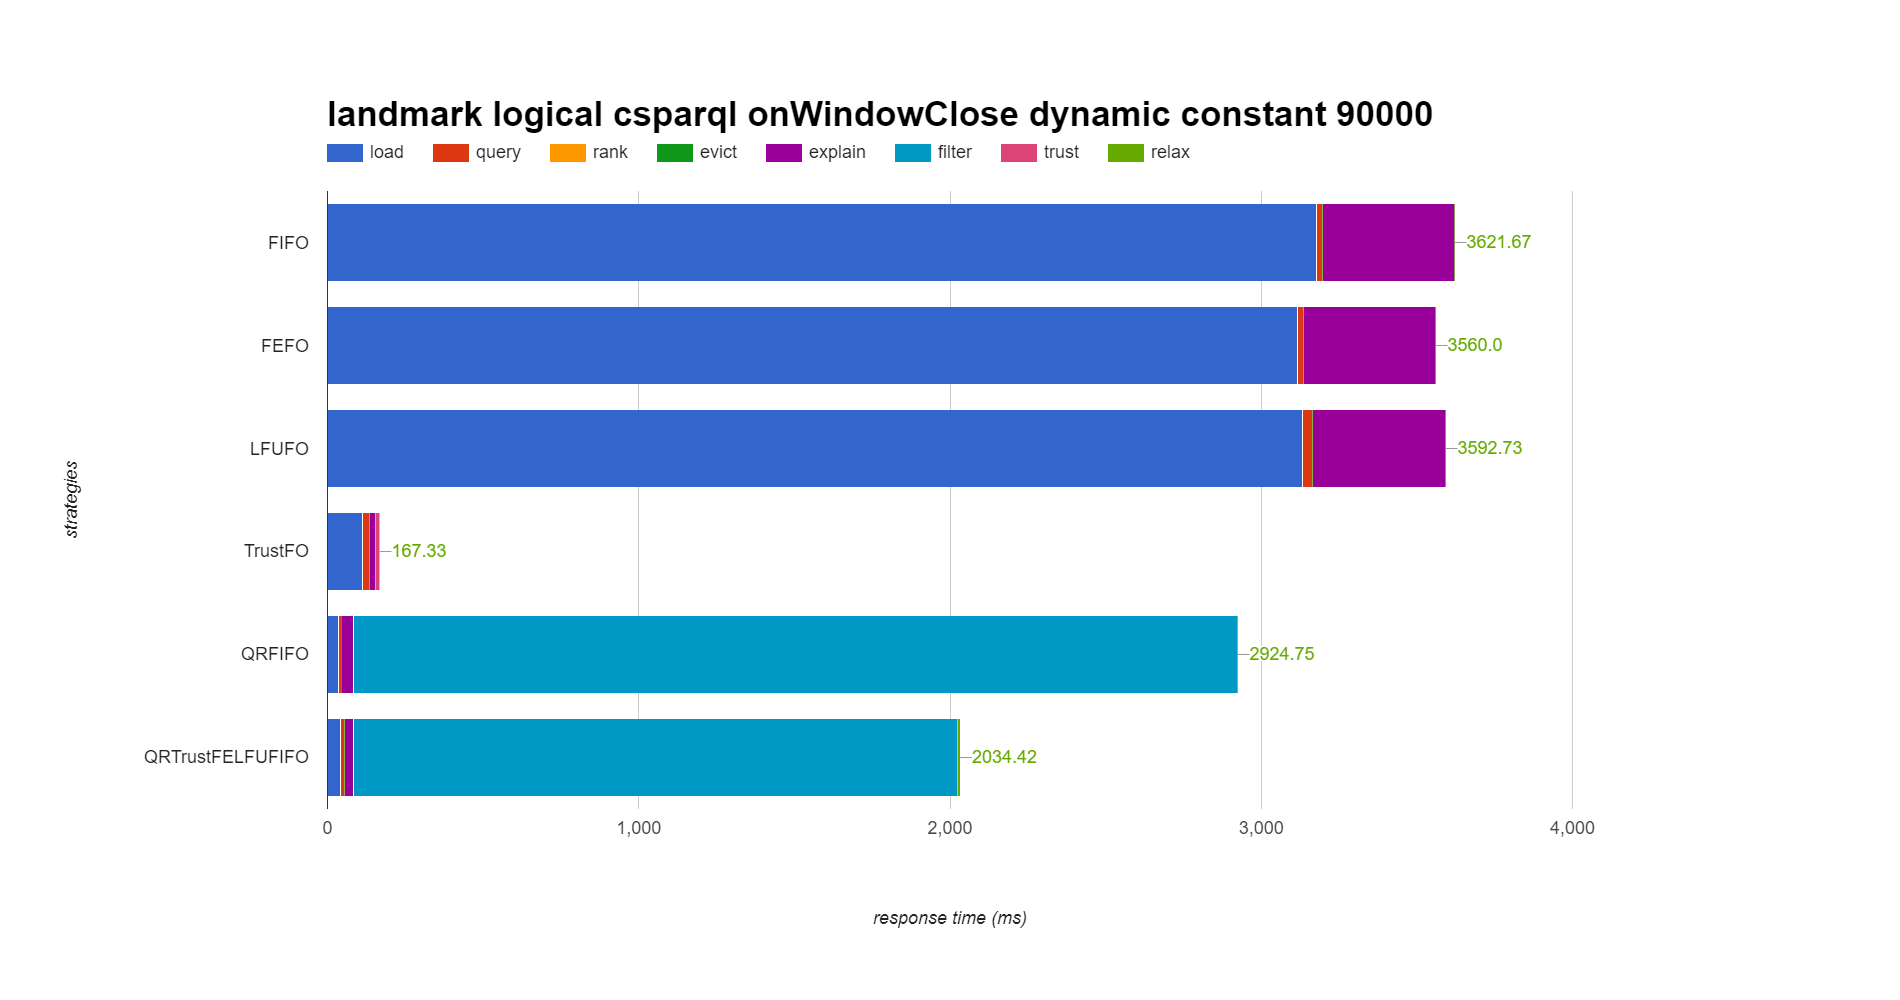
\includegraphics[width=6.5in]{img/6-9wt.png}
    \caption{Constant Stream Mode 90k Rate Response Time}
    \label{fig:6-csmrrt}
\end{figure}

In f mode though, things become some different. 
Since now the streaming rate is the peak value with 1/6 appearance probability, the average data items arrived is surely less than that in c mode. 
Thus all strategies can perform slightly better than what they do in c mode. 

\begin{figure}[!htbp]
	\centering
    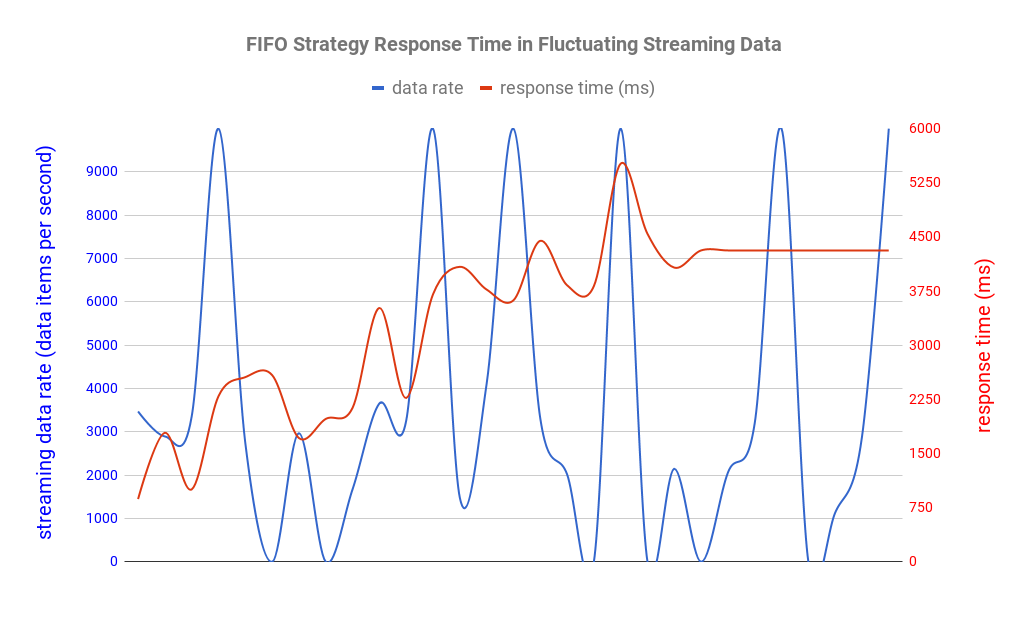
\includegraphics[width=5in]{img/6-fluctuating.png}
    \caption{FIFO Response Time Fluctuates with Stream Rate}
    \label{fig:6-fluc}
\end{figure}

\begin{figure}[!htbp]
	\centering
    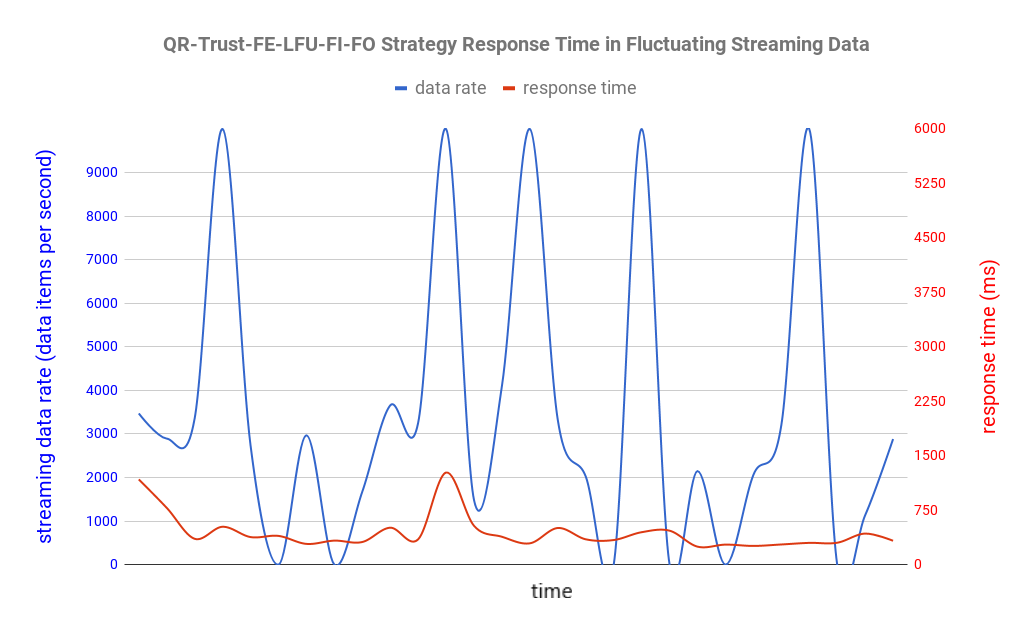
\includegraphics[width=5in]{img/6-flat.png}
    \caption{QR-Trust-FE-LFU-FI-FO Response Time is Stable}
   	\label{fig:6-flat}
\end{figure}

Figure \ref{fig:6-fluc} shows how FIFO's response time fluctuates with the streaming rate.
Stream reasoning system should be able to deal with stream bursts, which means that the system should not lose response when data behaves with a sudden large rate increase. 
Figure \ref{fig:6-flat} shows that semantic importance enabled window management strategy is able to keep a steady response time regardless of the streaming rate, which indicates that semantic importance is able to provide good system availability when facing versatile data streams. 
%
\subsection{Window}
Window is an important part of stream reasoning systems. 
SIGenBench is flexible in configuring different types of windows.
The results also show a significant relation between the window and the performance metrics.
This section introduces some observations and brings up some discussions. 
%
\subsubsection{Window Size}
Naively, the bigger the window size is, the more data it contains.
This means that the window can ``see'' a bigger snapshot of the data, which makes it possible to provide better performance in precision. 
However, the evaluation will show that this is not generally true, especially when the data expires quickly. 
Table \ref{tab:6-wes} shows the experiments setup.

\begin{table}[!htbp]
	\centering
    \caption{Window Experiment Setup}
    \label{tab:6-wes}
    \begin{tabular}{|c|l|} \hline
    \multicolumn{2}{|c|}{\textbf{experiment configuration}} \\ \hline
    window & report policy =``onWindowClose" \\ \hline
    data stream & \makecell[l]{lubm = 1 \\ sm = c (constant) \\ sr = 10000 data items/second \\ t = 3 (trust model 3)} \\ \hline
    query & \makecell[l]{CSPARQL target query \\ good query relevance filter query} \\ \hline
    \multicolumn{2}{|c|}{\textbf{experiment variable}} \\ \hline
    window & \makecell[l]{logical sliding window \\ window size = 1s, 3s, 5s, 7s, 9s \\ window step = 1s \\ strategy: FIFO, QR-FI-FO} \\ \cline{2-2}
           & \makecell[l]{logical lower-bounded landmark window \\ initial window size = 1s, 3s, 5s, 7s, 9s worth of data items \\ window step = 1s worth of data items \\ strategy: FIFO, QR-FI-FO, FE-FO, LFU-FO, Trust-FO \\ QR-Trust-FE-LFU-FI-FO} \\ \hline
    data expiration & \makecell[l]{ets = 1 quick expiration (1s to 3s) \\ ets = 2 normal expiration (3s to 7s) \\ ets = 3 slow expiration (7s to 10s) \\ ets = 4 implicit} \\ \hline
    \end{tabular}
\end{table}

\begin{center}
	\begin{longtable}{|c||c||c|c|c|c|c|}
	\caption[Sliding Window Size Performance]{Sliding Window Size Performance} \label{tab:6-swsp} \\
	\hline expiration & strategy & \makecell{window \\ size} & memory & \makecell{response \\ time} & precision & \makecell{through-\\put} \\ \hhline{|=#=#=|=|=|=|=|}
	\endfirsthead
	\multicolumn{7}{c} {{\bfseries \tablename\ \thetable{} -- continued from previous page}} \\
	\hline expiration & strategy & \makecell{window \\ size} & memory & \makecell{response \\ time} & precision & \makecell{through-\\put} \\ \hline 
	\endhead
	\hline \multicolumn{7}{|r|}{{Continued on next page}} \\ \hline
	\endfoot
	\hline
	\endlastfoot    
        quick & FIFO & 1s & 9999.10 & 2397.45 & 1 & 3816.67 \\ \cline{3-7}
			  &	     & 3s & 12506.25 & 2713.23 & 0 & 3969.17 \\ \cline{3-7}
			  &      & 5s & 16691.67 & 2816.50 & 0 & 4635.94 \\ \cline{3-7}
			  &      & 7s & 24997.75 & 3342.02 & 0 & 5416.76 \\ \cline{3-7}
			  &      & 9s & 49995.50 & 5517.47 & 0 & 5691.2 \\ \cline{2-7}
			  & QR-FI-FO & 1s & 13.90 & 413.81 & 1 & 31280.34 \\ \cline{3-7}
			  &		     & 3s & 27.00 & 292.25 & 1 & 37555.10 \\ \cline{3-7}
			  &          & 5s & 47.71 & 282.28 & 1 & 36745.25 \\ \cline{3-7}
			  &          & 7s & 69.80 & 305.25 & 1 & 33223.73 \\ \cline{3-7}
			  &          & 9s & 97.33 & 292.95 & 1 & 34335.72 \\ \hhline{|=#=#=|=|=|=|=|}
        normal & FIFO & 1s & 9999.10 & 2486.20 & 0.8 & 3578.65 \\ \cline{3-7}
			   &	  & 3s & 12498.88 & 2732.78 & 1 & 3826.70 \\ \cline{3-7}
			   &      & 5s & 16665.17 & 3028.36 & 0 & 4254.73 \\ \cline{3-7}
			   &      & 7s & 24997.75 & 3230.50 & 0 & 5326.08 \\ \cline{3-7}
			   &      & 9s & 49995.50 & 4990.23 & 0 & 6035.96 \\ \cline{2-7}
			   & QR-FI-FO & 1s & 14.00 & 532.62 & 1 & 24508.78 \\ \cline{3-7}
			   &		  & 3s & 29.62 & 271.65 & 1 & 39502.95 \\ \cline{3-7}
			   &          & 5s & 48.00 & 263.85 & 1 & 38786.65 \\ \cline{3-7}
			   &          & 7s & 75.00 & 281.03 & 1 & 35005.22 \\ \cline{3-7}
			   &          & 9s & 97.67 & 294.49 & 1 & 34277.19 \\ \hhline{|=#=#=|=|=|=|=|}
        slow  & FIFO & 1s & 9999.1 & 2489.96 & 1 & 3820.44 \\ \cline{3-7}
			  &	     & 3s & 12498.88 & 2716.76 & 1& 3939.00 \\ \cline{3-7}
			  &      & 5s & 16665.17 & 2994.14 & 1& 4356.12 \\ \cline{3-7}
			  &      & 7s & 24997.75 & 3283.32 & 1& 5392.64 \\ \cline{3-7}
			  &      & 9s & 49995.50 & 4906.29 & 1& 6294.06 \\ \cline{2-7}
			  & QR-FI-FO & 1s & 13.80 & 476.61 & 1 & 24921.91 \\ \cline{3-7}
			  &		     & 3s & 28.50 & 272,70 & 1 & 39057.89 \\ \cline{3-7}
			  &          & 5s & 47.14 & 273.08 & 1 & 36624.77 \\ \cline{3-7}
			  &          & 7s & 70.20 & 269.89 & 1 & 36785.58 \\ \cline{3-7}
			  &          & 9s & 96.67 & 284.10 & 1 & 36531.61 \\ \hhline{|=#=#=|=|=|=|=|}
        none   & FIFO & 1s & 9999.10 & 2307.75 & 1 & 3919.80 \\ \cline{3-7}
			   &	  & 3s & 12498.88 & 2587.18 & 1 & 4106.65 \\ \cline{3-7}
			   &      & 5s & 16665.17 & 2928.87 & 1 & 4496.00 \\ \cline{3-7}
			   &      & 7s & 19998.20 & 2876.45 & 1 & 5260.03 \\ \cline{3-7}
			   &      & 9s & 49995.50 & 4704.67 & 1 & 6653.98 \\ \cline{2-7}
			   & QR-FI-FO & 1s & 13.90 & 683.52 & 1 & 18572.88\\ \cline{3-7}
			   &		  & 3s & 28.25 & 276.81 & 1 & 39690.09\\ \cline{3-7}
			   &          & 5s & 49.57 & 274.90 & 1 & 39302.19\\ \cline{3-7}
			   &          & 7s & 72.80 & 281.03 & 1 & 37639.46\\ \cline{3-7}
			   &          & 9s & 97.00 & 283.03 & 1 & 36268.04 \\              
\end{longtable}
    \begin{tablenotes}
 		\item memory unit: number of data items
 		\item response time unit: ms
 		\item throughput unit: data items/second
    \end{tablenotes}
\end{center}

\begin{center}
	\begin{longtable}{|c||c||c|c|c|c|c|}
	\caption[Landmark Window Size Performance]{Landmark Window Size Performance} \label{tab:6-lwsp} \\
	\hline expiration & strategy & \makecell{window \\ size} & memory & \makecell{response \\ time} & precision & \makecell{through-\\put} \\ \hhline{|=#=#=|=|=|=|=|}
	\endfirsthead
	\multicolumn{7}{c} {{\bfseries \tablename\ \thetable{} -- continued from previous page}} \\
	\hline expiration & strategy & \makecell{window \\ size} & memory & \makecell{response \\ time} & precision & \makecell{through-\\put} \\ \hline 
	\endhead
	\hline \multicolumn{7}{|r|}{{Continued on next page}} \\ \hline
	\endfoot
	\hline
	\endlastfoot    
        quick & FIFO & 1s & 9999.10 & 2430.96 & 0.50 & 3752.29 \\ \cline{3-7}
			  &	     & 3s & 12498.88 & 2774.65 & 0 & 3795.21 \\ \cline{3-7}
			  &      & 5s & 16665.17 & 2818.66 & 0 & 4588.54 \\ \cline{3-7}
			  &      & 7s & 24997.75 & 3359.35 & 0 & 5153.53 \\ \cline{3-7}
			  &      & 9s & 49995.50 & 4847.37 & 0 & 6298.00 \\ \cline{2-7}
			  & QR-FI-FO & 1s & 14.00 & 284.13 & 1& 38445.51\\ \cline{3-7}
			  &		     & 3s & 28.50 & 281.85 & 1& 37866.29\\ \cline{3-7}
			  &          & 5s & 51.67 & 281.55 & 1& 37681.78\\ \cline{3-7}
			  &          & 7s & 75.00 & 308.26 & 1& 33850.17\\ \cline{3-7}
			  &          & 9s & 101.33 & 305.02 & 1& 36505.08\\ \cline{2-7}
			  & FE-FO & 1s & 10756.00 & 2531.39 & 0.50 & 3541.09 \\ \cline{3-7}
			  &		  & 3s & 12498.88 & 2691.70 & 1 & 3931.45 \\ \cline{3-7}
			  &       & 5s & 16665.17 & 2897.93 & 0 & 4484.57 \\ \cline{3-7}
			  &       & 7s & 24997.75 & 3336.05 & 0 & 5185.42 \\ \cline{3-7}
			  &       & 9s & 49995.50 & 4747.63 & 0 & 6456.97 \\ \cline{2-7}
			  & LFU-FO & 1s & 10045.40 & 2132.99 & 0.50 & 1938.02 \\ \cline{3-7}
			  &		   & 3s & 12541.50 & 2279.74 & 0 & 2072.37 \\ \cline{3-7}
			  &        & 5s & 16717.17 & 2578.32 & 0 & 2390.56 \\ \cline{3-7}
			  &        & 7s & 25054.50 & 3175.83 & 0 & 3084.56 \\ \cline{3-7}
			  &        & 9s & 50044.50 & 4664.32 & 0 & 4838.07 \\ \cline{2-7}
			  & Trust-FO & 1s & 633.70 & 103.04 & 1 & 50698.44\\ \cline{3-7}
			  &			 & 3s & 3663.12 & 188.17 & 1& 41681.18\\ \cline{3-7}
			  &          & 5s & 1727.67 & 148.26 & 1& 57547.22\\ \cline{3-7}
			  &          & 7s & 2911.50 & 170.09 & 1& 75533.43\\ \cline{3-7}
			  &          & 9s & 4298.00 & 205.83 & 1& 115557.47\\ \cline{2-7}
              & QR-Trust- & 1s & 23.80 & 280.54 & 1& 36373.01\\ \cline{3-7}
			  &	FE-LFU-   & 3s & 27.38 & 280.88 & 1& 38139.23\\ \cline{3-7}
			  & FI-FO     & 5s & 30.29 & 283.78 & 1& 38226.24\\ \cline{3-7}
			  &           & 7s & 41.40 & 298.30 & 1& 37966.39\\ \cline{3-7}
			  &           & 9s & 53.00 & 289.23 & 1& 41373.43\\ \hhline{|=#=#=|=|=|=|=|}
        normal & FIFO & 1s & 9999.10 & 2419.96 & 0.80 & 3667.82 \\ \cline{3-7}
			   &	  & 3s & 12498.88 & 2674.31 & 0.67 & 3837.80 \\ \cline{3-7}
			   &      & 5s & 16683.33 & 3000.33 & 0 & 4305.57 \\ \cline{3-7}
			   &      & 7s & 24997.75 & 3265.81 & 0 & 5274.38 \\ \cline{3-7}
			   &      & 9s & 49995.50 & 4582.60 & 0 & 6670.76 \\ \cline{2-7}
			   & QR-FI-FO & 1s & 14.00 & 266.50 & 1 & 40456.74 \\ \cline{3-7}
			   &		  & 3s & 29.75 & 274.62 & 1 & 39103.46\\ \cline{3-7}
			   &          & 5s & 48.14 & 271.19 & 1 & 37909.13 \\ \cline{3-7}
			   &          & 7s & 76.20 & 279.30 & 1 & 35815.82 \\ \cline{3-7}
			   &          & 9s & 97.00 & 279.83 & 1 & 37002.21 \\ \cline{2-7}
			   & FE-FO & 1s & 13623.80 & 2463.58 & 1 & 3373.77 \\ \cline{3-7}
			   &	   & 3s & 15852.12 & 2736.27 & 1 & 3667.55 \\ \cline{3-7}
			   &       & 5s & 18404.50 & 3085.17 & 0 & 4192.63 \\ \cline{3-7}
			   &       & 7s & 24997.75 & 3264.10 & 0 & 5285.47 \\ \cline{3-7}
			   &       & 9s & 49995.50 & 4749.43 & 1 & 6437.54 \\ \cline{2-7}
			   & LFU-FO & 1s & 10048.00 & 2057.90 & 1 & 2093.87 \\ \cline{3-7}
			   &		& 3s & 12533.12 & 2313.39 & 1 & 2214.87 \\ \cline{3-7}
			   &        & 5s & 16707.50 & 2599.38 & 0 & 2497.70 \\ \cline{3-7}
			   &        & 7s & 25046.25 & 3091.38 & 0 & 3180.38 \\ \cline{3-7}
			   &        & 9s & 50035.50 & 4554.67 & 0 & 4853.48 \\ \cline{2-7}
			   & Trust-FO & 1s & 621.10 & 105.11 & 1 & 51929.24\\ \cline{3-7}
			   &		  & 3s & 3632.88 & 179.74 & 1& 43540.49\\ \cline{3-7}
			   &          & 5s & 1720.17 & 140.26 & 1& 60236.67\\ \cline{3-7}
			   &          & 7s & 2927.25 & 179.86 & 1& 72851.45\\ \cline{3-7}
			   &          & 9s & 4350.50 & 207.43 & 1& 119400.24\\ \cline{2-7}
               & QR-Trust- & 1s & 49.20 & 276.39 & 1 & 34300.58\\ \cline{3-7}
			   & FE-LFU-   & 3s & 56.62 & 267.66 & 1 & 35337.43\\ \cline{3-7}
			   & FI-FO     & 5s & 58.86 & 277.59 & 1 & 35474.59\\ \cline{3-7}
			   &           & 7s & 63.80 & 289.14 & 1 & 35905.36\\ \cline{3-7}
			   &           & 9s & 73.33 & 280.02 & 1 & 39179.66\\ \hhline{|=#=#=|=|=|=|=|}
        slow  & FIFO & 1s & 9999.10 & 2495.20 & 1 & 3815.66 \\ \cline{3-7}
			  &	     & 3s & 12498.88 & 2758.74 & 1 & 3789.91 \\ \cline{3-7}
			  &      & 5s & 16665.17 & 3033.92 & 1 & 4334.53 \\ \cline{3-7}
			  &      & 7s & 24997.75 & 3298.89 & 1 & 5377.64 \\ \cline{3-7}
			  &      & 9s & 49995.50 & 4734.86 & 1 & 6611.63 \\ \cline{2-7}
			  & QR-FI-FO & 1s & 13.80 & 263.60 & 1 & 41068.22 \\ \cline{3-7}
			  &		     & 3s & 27.38 & 257.78 & 1 & 41135.43 \\ \cline{3-7}
			  &          & 5s & 46.71 & 266.54 & 1 & 37471.11 \\ \cline{3-7}
			  &          & 7s & 73.00 & 273.52 & 1 & 36718.41 \\ \cline{3-7}
			  &          & 9s & 96.67 & 265.43 & 1 & 39118.68 \\ \cline{2-7}
			  & FE-FO & 1s & 17786.00 & 2614.28 & 1 & 3063.04 \\ \cline{3-7}
			  &		  & 3s & 20244.25 & 2907.29 & 1 & 3336.60 \\ \cline{3-7}
			  &       & 5s & 24809.00 & 3263.75 & 1 & 3616.50 \\ \cline{3-7}
			  &       & 7s & 29148.25 & 3436.78 & 1 & 5034.55 \\ \cline{3-7}
			  &       & 9s & 51284.00 & 4785.86 & 1 & 6618.06 \\ \cline{2-7}
			  & LFU-FO & 1s & 12256.30 & 2180.53 & 1 & 2118.27\\ \cline{3-7}
			  &		   & 3s & 12529.62 & 2297.83 & 1 & 2279.03 \\ \cline{3-7}
			  &        & 5s & 16701.83 & 2592.45 & 1 & 2591.91 \\ \cline{3-7}
			  &        & 7s & 25035.25 & 3127.57 & 1 & 3288.47 \\ \cline{3-7}
			  &        & 9s & 50024.00 & 4648.54 & 1 & 5091.41 \\ \cline{2-7}
			  & Trust-FO & 1s & 644.70 & 109.56 & 1 & 52009.83 \\ \cline{3-7}
			  &			    & 3s & 3726.50 & 195.68 & 1& 42545.49\\ \cline{3-7}
			  &             & 5s & 1740.17 & 148.78 & 1& 59877.90\\ \cline{3-7}
			  &             & 7s & 2938.00 & 184.45 & 1& 73760.09\\ \cline{3-7}
			  &          & 9s & 4344.50 & 205.12 & 1& 118976.33\\ \cline{2-7}
              & QR-Trust- & 1s & 64.00 & 268.07 & 1& 31875.40 \\ \cline{3-7}
			  &	FE-LFU-   & 3s & 75.62 & 260.77 & 1& 32973.11 \\ \cline{3-7}
			  & FI-FO     & 5s & 80.14 & 274.95 & 1& 32462.06 \\ \cline{3-7}
			  &           & 7s & 89.80 & 276.26 & 1& 33907.25 \\ \cline{3-7}
			  &           & 9s & 99.33 & 268.83 & 1& 38386.79 \\ \hhline{|=#=#=|=|=|=|=|}
        none   & FIFO & 1s & 9999.10 & 2294.27 & 1 & 3948.59 \\ \cline{3-7}
			   &	  & 3s & 12498.88 & 2602.75 & 1 & 3994.08 \\ \cline{3-7}
			   &      & 5s & 16665.17 & 3020.46 & 1 & 4367.48 \\ \cline{3-7}
			   &      & 7s & 24997.75 & 3235.59 & 1 & 5495.22 \\ \cline{3-7}
			   &      & 9s & 49995.50 & 4540.93 & 1 & 7001.04 \\ \cline{2-7}
			   & QR-FI-FO & 1s & 13.90 & 252.62 & 1 & 43018.83 \\ \cline{3-7}
			   &		  & 3s & 28.62 & 270.16 & 1 & 40294.59 \\ \cline{3-7}
			   &          & 5s & 49.57 & 279.72 & 1 & 38342.87 \\ \cline{3-7}
			   &          & 7s & 73.00 & 267.42 & 1 & 39088.26 \\ \cline{3-7}
			   &          & 9s & 97.00 & 271.25 & 1 & 39286.83 \\ \cline{2-7}
 			   & FE-FO\footnote{FE-FO can not run because of no data expiration.} & 1s & - & - & - & - \\ \cline{3-7}
			   &	   & 3s & - & - & - & - \\ \cline{3-7}
			   &       & 5s & - & - & - & - \\ \cline{3-7}
			   &       & 7s & - & - & - & - \\ \cline{3-7}
			   &       & 9s & - & - & - & - \\ \cline{2-7}
			   & LFU-FO & 1s & 10043.10 & 2088.77 & 1 & 1963.50 \\ \cline{3-7}
			   &		& 3s & 12533.25 & 2266.74 & 1 & 2091.60 \\ \cline{3-7}
			   &        & 5s & 16706.17 & 2557.57 & 1 & 2395.06 \\ \cline{3-7}
			   &        & 7s & 24043.50 & 3052.05 & 1 & 3083.90 \\ \cline{3-7}
			   &        & 9s & 50031.50 & 4666.90 & 1 & 4700.31 \\ \cline{2-7}
			   & Trust-FO & 1s & 638.20 & 108.65 & 1& 52334.72 \\ \cline{3-7}
			   &			 & 3s & 3705.00 & 199.62 & 1& 42599.58 \\ \cline{3-7}
			   &             & 5s & 1727.83 & 147.46 & 1& 61004.25 \\ \cline{3-7}
			   &             & 7s & 2929.50 & 164.79 & 1& 77156.56 \\ \cline{3-7}
			   &          & 9s & 4337.00 & 222.00 & 1& 111829.81 \\ \cline{2-7}
              & QR-Trust- & 1s & 34.70 & 264.92 & 1 & 30697.71 \\ \cline{3-7}
			  &	FE-LFU-   & 3s & 39.25 & 258.48 & 1 & 31684.53 \\ \cline{3-7}
			  & FI-FO     & 5s & 45.83 & 262.53 & 1 & 32078.81 \\ \cline{3-7}
			  &           & 7s & 42.60 & 271.61 & 1 & 32704.94 \\ \cline{3-7}
			  &           & 9s & 61.00 & 266.88 & 1 & 36624.77 \\
\end{longtable}
    \begin{tablenotes}
 		\item memory unit: number of data items
 		\item response time unit: ms
 		\item throughput unit: data items/second
    \end{tablenotes}
\end{center}

Table \ref{tab:6-swsp} shows sliding window size performance. 
Only two strategies FIFO and QR-FI-FO are employed so as to maintain the integrity of the sliding window semantics. 

FIFO tends to consume much more memory than QR-FI-FO in all scenarios. 
Both strategies consume more memory as the window size increases. 
QR-FI-FO manages to keep the response time within 1 second, while FIFO's response time increases as the window size increases. 
When data expires quickly, FIFO's precision drops as window size increases.
As data expires slowly, FIFO is able to keep a good precision. 
QR-FI-FO's precision is always 1, regardless how data expires or window size is. 
FIFO's throughput is way less than that of QR-FI-FO, in fact FIFO's throughput is less than the streaming rate.

Table \ref{tab:6-lwsp} shows the performance of landmark window size. 
Lower-bounded landmark window will only have its upper bound proceeds. 
According to the extended window semantics, the window definition sets the initial window size of a lower-bounded window size. 
FIFO and QR-FI-FO's performance is quite similar as in Table \ref{tab:6-swsp}. 
It can also be seen that FE-FO and LFU-FO performs similar as FIFO. 
Strategies with QR or trust aspect is capable to perform well even if window size increases. 
The compound strategy QR-Trust-FE-LFU-FI-FO shows a good performance as well. 

The results show a strong correlation among the four metrics: the strategy will perform better as long as the memory consumption is small.
With a small amount of data items in the window, response time will be fast, thus the system is able to keep up with the streaming data rate and expiration, thus the precision and throughput are improved. 
Data expiration also plays an important role for strategy performance. 
Strategies that can manage data in a fast speed can keep up with fast data expiration, which is the main reason to achieve the precision of 1. 
As the data expires slowly, all strategies can deliver good precision, because the data expiration is more tolerant with longer system processing time.
%
\subsubsection{Report Policy}
Report policies are part of window semantics. 
They determine the condition to fire the query and report the results.
They are also part of the reasons to explain the different results reported by different stream reasoning engines \cite{dell2013correctness}. 
%
\subsubsection{Strategy}
Different window management strategies are supported by different combinations of semantic importance aspects, which views data importance in different ways, thus can provide different results and performances. 
However, the performance of any strategy is not only dependent on its semantic importance aspects, but also the environment it is deployed. 
For example, if the streaming data carries its own trust score, it is generally a good idea to add the trustworthiness in the strategy. 
In all ways, query relevance filtering is recommended because of its huge positive influence to the system performance.
The reason to enable so many possible strategies from semantic importance is to allow the flexibility of choosing an appropriate one that can work well in a specific use case. 
This requires the users to be aware of the traits in their own use cases, as well as the performance impacts by different semantic importance aspect.
The above experiments have already shown all the strategies' performances under different scenarios.
%
\section{Summary}
The above experiments have illustrated that SIGenBench is both powerful and flexible to generalize and benchmark semantic importance. 
Query relevance can significantly increase the strategy performance as in Table \ref{tab:6-qrp}.
A good query relevance can comprehensively improve stream reasoning systems.
Even an OK or bad query relevance can still improve system response time. 
However, it can also be seen that as streaming rate increases, query relevance can reach the limitation where filtering time can take too long, which can negatively impact the response time and precision. 
Temporal provenance, especially the expiration timestamp, is suitable where data carries explicit expiration timestamps. 
They are good at picking up expired data to avoid invalid query results. 
However, in order to guarantee system response time, the experimental results recommend to work with QR aspect. 
Query participation, although does not show an outstanding performance improvement, is still an important aspect. 
It is able to keep the partial necessary data items and wait for the other necessary data items to answer the query, which can improve system precision. 
From the experiment results, it is recommended to work with QR to improve system metrics, as well as temporal provenance if explicit expiration timestamps are carried. 
Trustworthiness is very straightforward. 
It relies trust models to assign numerical trust scores, based on which the data can be ranked. 
The experimental results have shown that different trust models can yield different system results. 
The algorithm to rank trust scores only takes O(n), where n is the number of data items in the window. 
This means trust aspect can run much faster, thus it is recommended to consider trustworthiness when data carries trust scores. 
Finally, a compound strategy like QR-Trust-FE-LFU-FI-FO considers multiple importance factors, and achieves far better performance than FIFO. 
This finding has already proves that semantic importance enabled window management strategies are able to improve the stream reasoning systems. 